% Preamble-ish commands {{{
\newcommand{\sectionbreak}{\clearpage}
\renewcommand*{\thefigure}{S\arabic{figure}}
\renewcommand*{\thetable}{S\arabic{table}}
\renewcommand*{\thepage}{S\arabic{page}}
\setcounter{page}{1}
\setcounter{figure}{0}
\setcounter{table}{0}
\onehalfspacing
% }}}
% Title page {{{
\hspace{0pt}
\vfill
\begin{center}
    \huge
    Supporting Information

    \textit{for}

    Diversifying NOAH Supersequences with New HSQC-based Modules

    \vspace{1cm}

    \Large Jonathan R. J. Yong,\textsuperscript{1} {\=E}riks Kup{\v{c}}e,\textsuperscript{2} Tim D. W. Claridge\textsuperscript{1,}*

    \vspace{1cm}

    \large \textsuperscript{1} \textit{Chemistry Research Laboratory, Department of Chemistry, University of Oxford, Mansfield Road, Oxford, OX1 3TA, U.K.}

    \textsuperscript{2} \textit{Bruker UK Ltd., Banner Lane, Coventry, CV4 9GH, U.K.}

    * \texttt{tim.claridge@chem.ox.ac.uk}
\end{center}
\thispagestyle{empty}
\vfill
\hspace{0pt}
\newpage
%}}}

% Table of contents {{{
\tableofcontents

\newpage
%}}}

\section{Product operator analysis for NOAH modules}

\begin{figure}
    \centering
    % Inkscape
    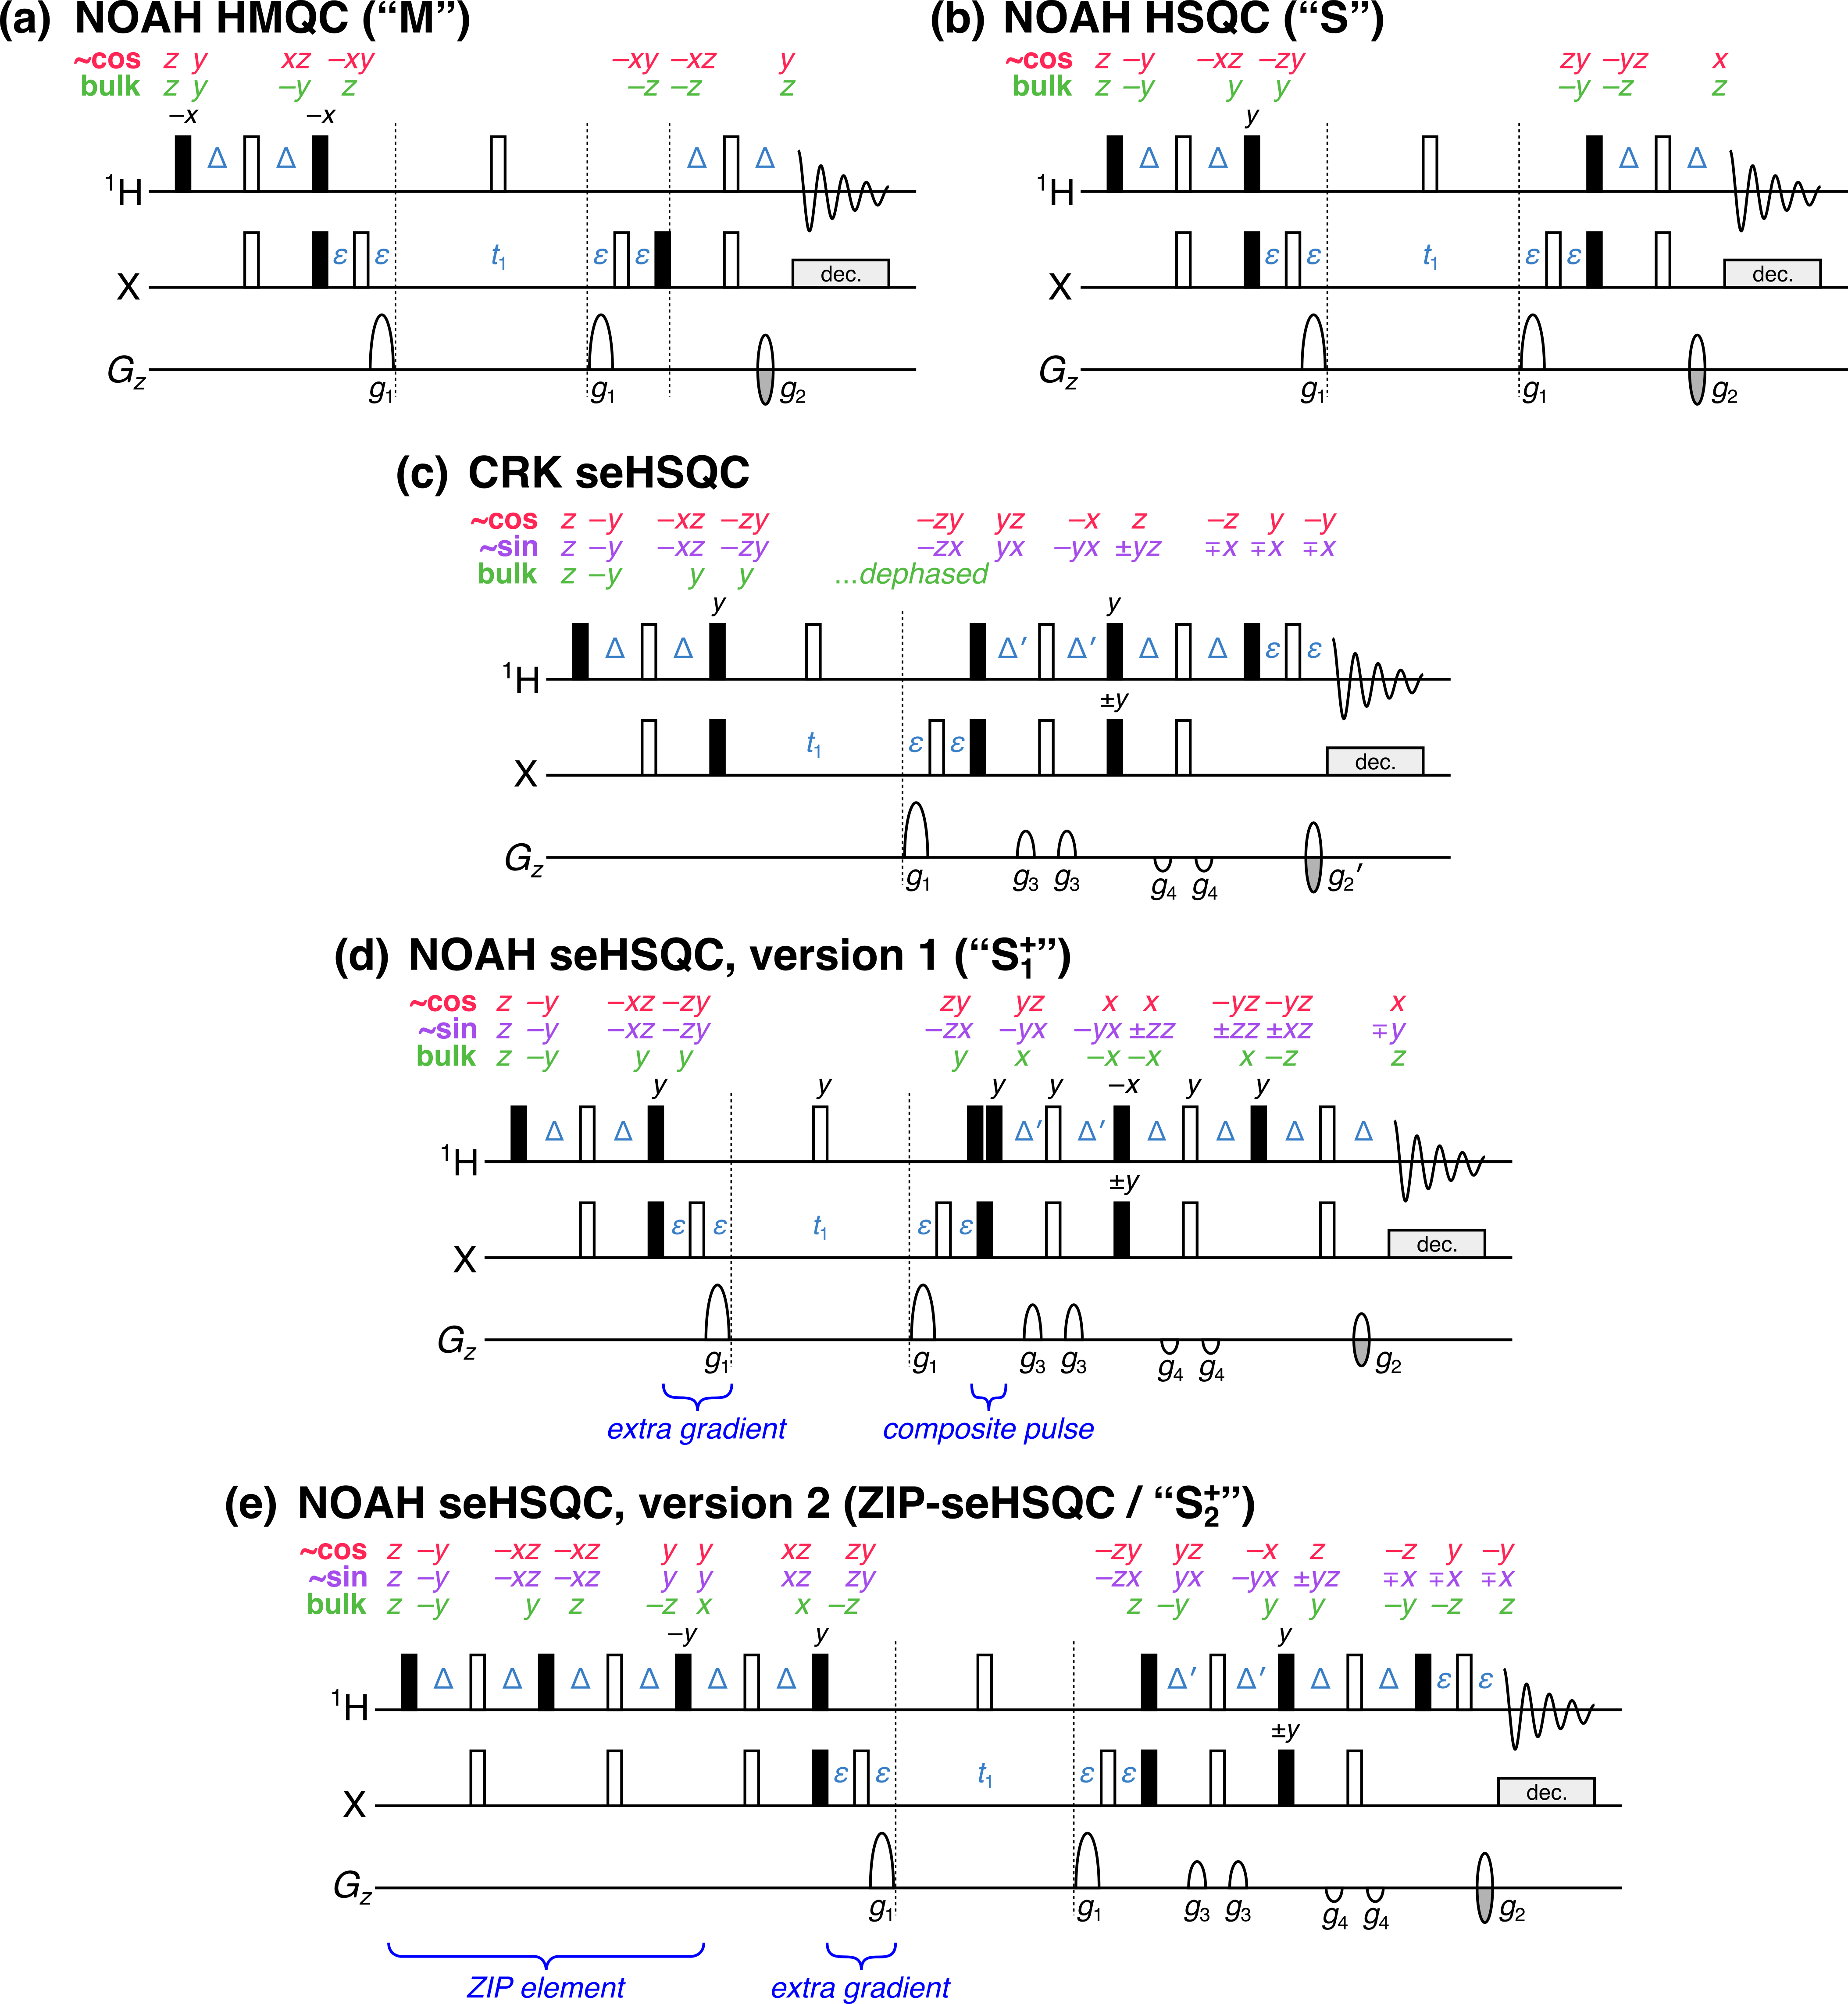
\includegraphics[width=0.8\textwidth]{./figures/pprogs_prodop.png}
    \caption{
        Product operators present at each stage of NOAH modules for an IS spin system.
        One-letter terms $m$ ($m \in \{x, y, z\}$) are shorthand for single-spin terms on proton, i.e.\ $\hat{I}_m$.
        Two-letter terms $mn$ are shorthand for two-spin terms on both the proton and heteronucleus, i.e.\ $2\hat{I}_m\hat{S}_n$.
        ``$\sim$cos'' represents the pathway for directly coupled proton magnetisation that is cosine-modulated after $t_1$: for the HMQC and HSQC, this is the only component that is detected.
        For the seHSQC, the sine-modulated component (labelled with ``$\sim$sin'') is also detected.
        ``bulk'' refers to the bulk magnetisation, i.e.\ protons that are not directly coupled to the heteronucleus.
        \textbf{(a)} NOAH HMQC.
        \textbf{(b)} NOAH HSQC.
        \textbf{(c)} NOAH seHSQC with ISR.
        Immediately following the ISR pulse sequence element, directly bonded protons are rotated onto $+y$, whereas the bulk magnetisation is rotated onto $+x$.
        Note that this analysis assumes $\Delta' = 1/(4\cdot\onejxh)$.
    }
    \label{fig:pprogs_prodop}
\end{figure}

\section{Multiplicity editing in seHSQC}

\begin{figure}
    \centering
    % done in Inkscape
    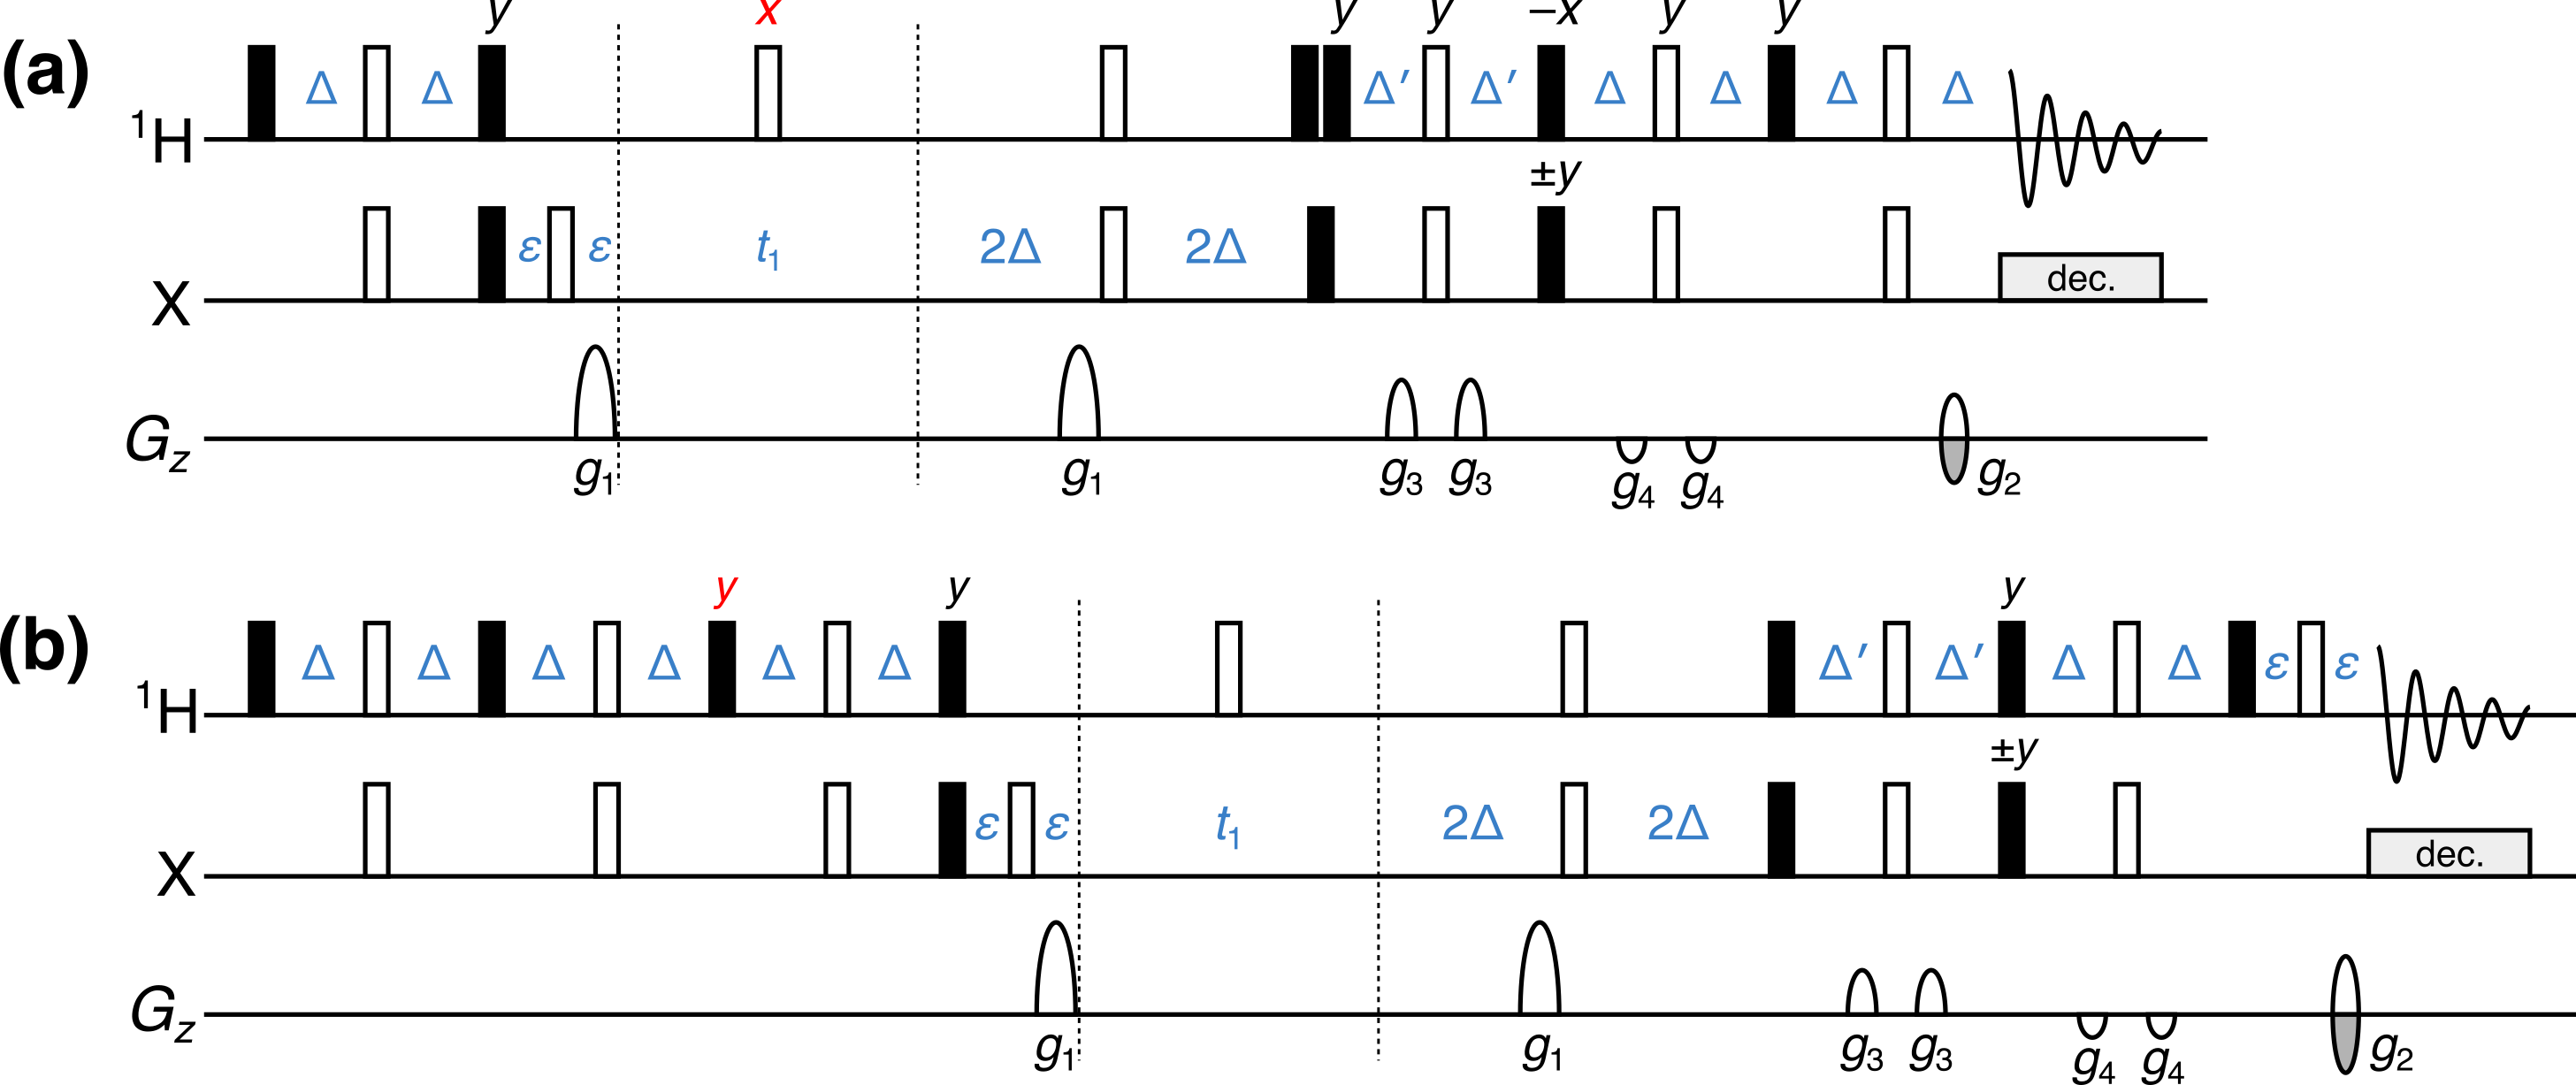
\includegraphics[width=0.8\textwidth]{./figures/mult_edit.png}
    \caption{
        Implementation of multiplicity editing in the new NOAH seHSQC module.
        Note the different phase in the third \proton{} \ang{90} pulse ($+y$ as opposed to the $-y$ in \figref{pprogs_prodop}c).
        This is needed to compensate for the extra \proton{} \ang{180} pulse in the editing period.
        Symbols have the same meaning as in \figref{pprogs} of the main text.
    }
    \label{fig:edited_sehsqc_pprog}
\end{figure}

\begin{figure}
    \centering
    % figures/edited_sn_comp.py
    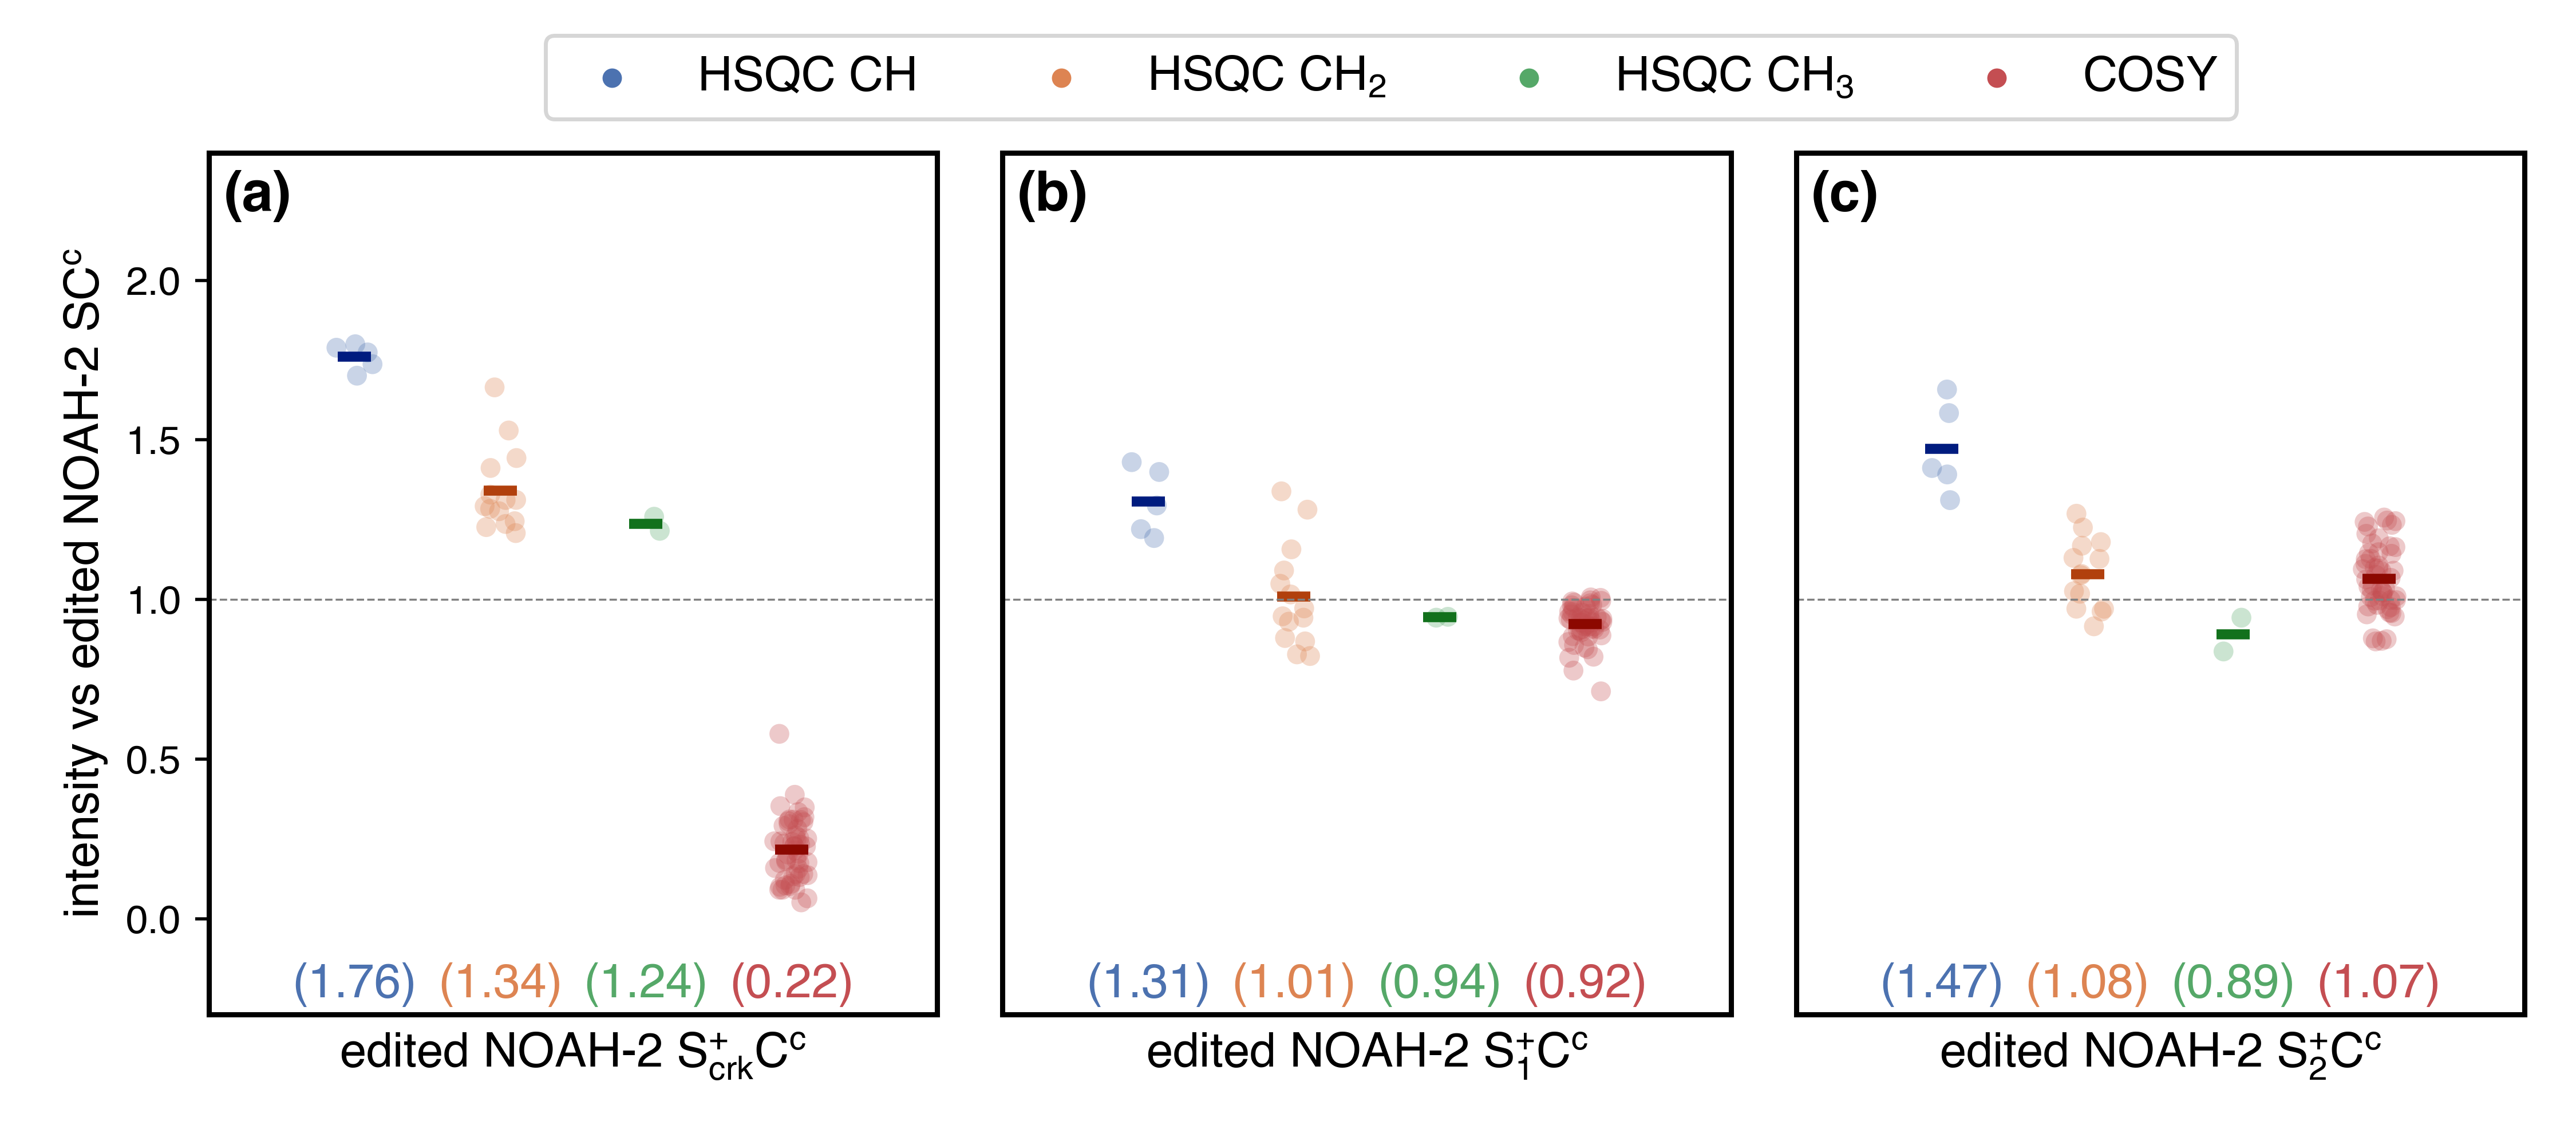
\includegraphics[width=0.8\textwidth]{./figures/edited_sn_comp.png}
    \caption{
        Sensitivity of edited seHSQC versus the NOAH HSQC/CLIP-COSY supersequence.
        \textbf{(a)} CRK edited seHSQC + CLIP-COSY.
        Although larger gains are observed in the HSQC, the COSY intensities are severely decreased.
        \textbf{(b)} NOAH edited seHSQC + CLIP-COSY.
        On average, sensitivity gains are observed in both the HSQC and COSY modules (except for HSQC \ce{CH3} peaks).
        \andro{}
    }
    \label{fig:edited_sn_comp}
\end{figure}

\section{Effect of setting \texorpdfstring{$\Delta' = 1/(4\cdot\onejch)$}{Delta' = 1/(4*1JCH)} in seHSQC}

The $\Delta'$ delay in the CRK and NOAH seHSQC sequences can be set to $1/(4\cdot\onejch)$ in order to optimise the sensitivity enhancement for \ce{CH} groups only.
The effects of doing so are shown here for the unedited and edited seHSQCs respectively.

\begin{figure}
    \centering
    % figures/combined_1_4j.py
    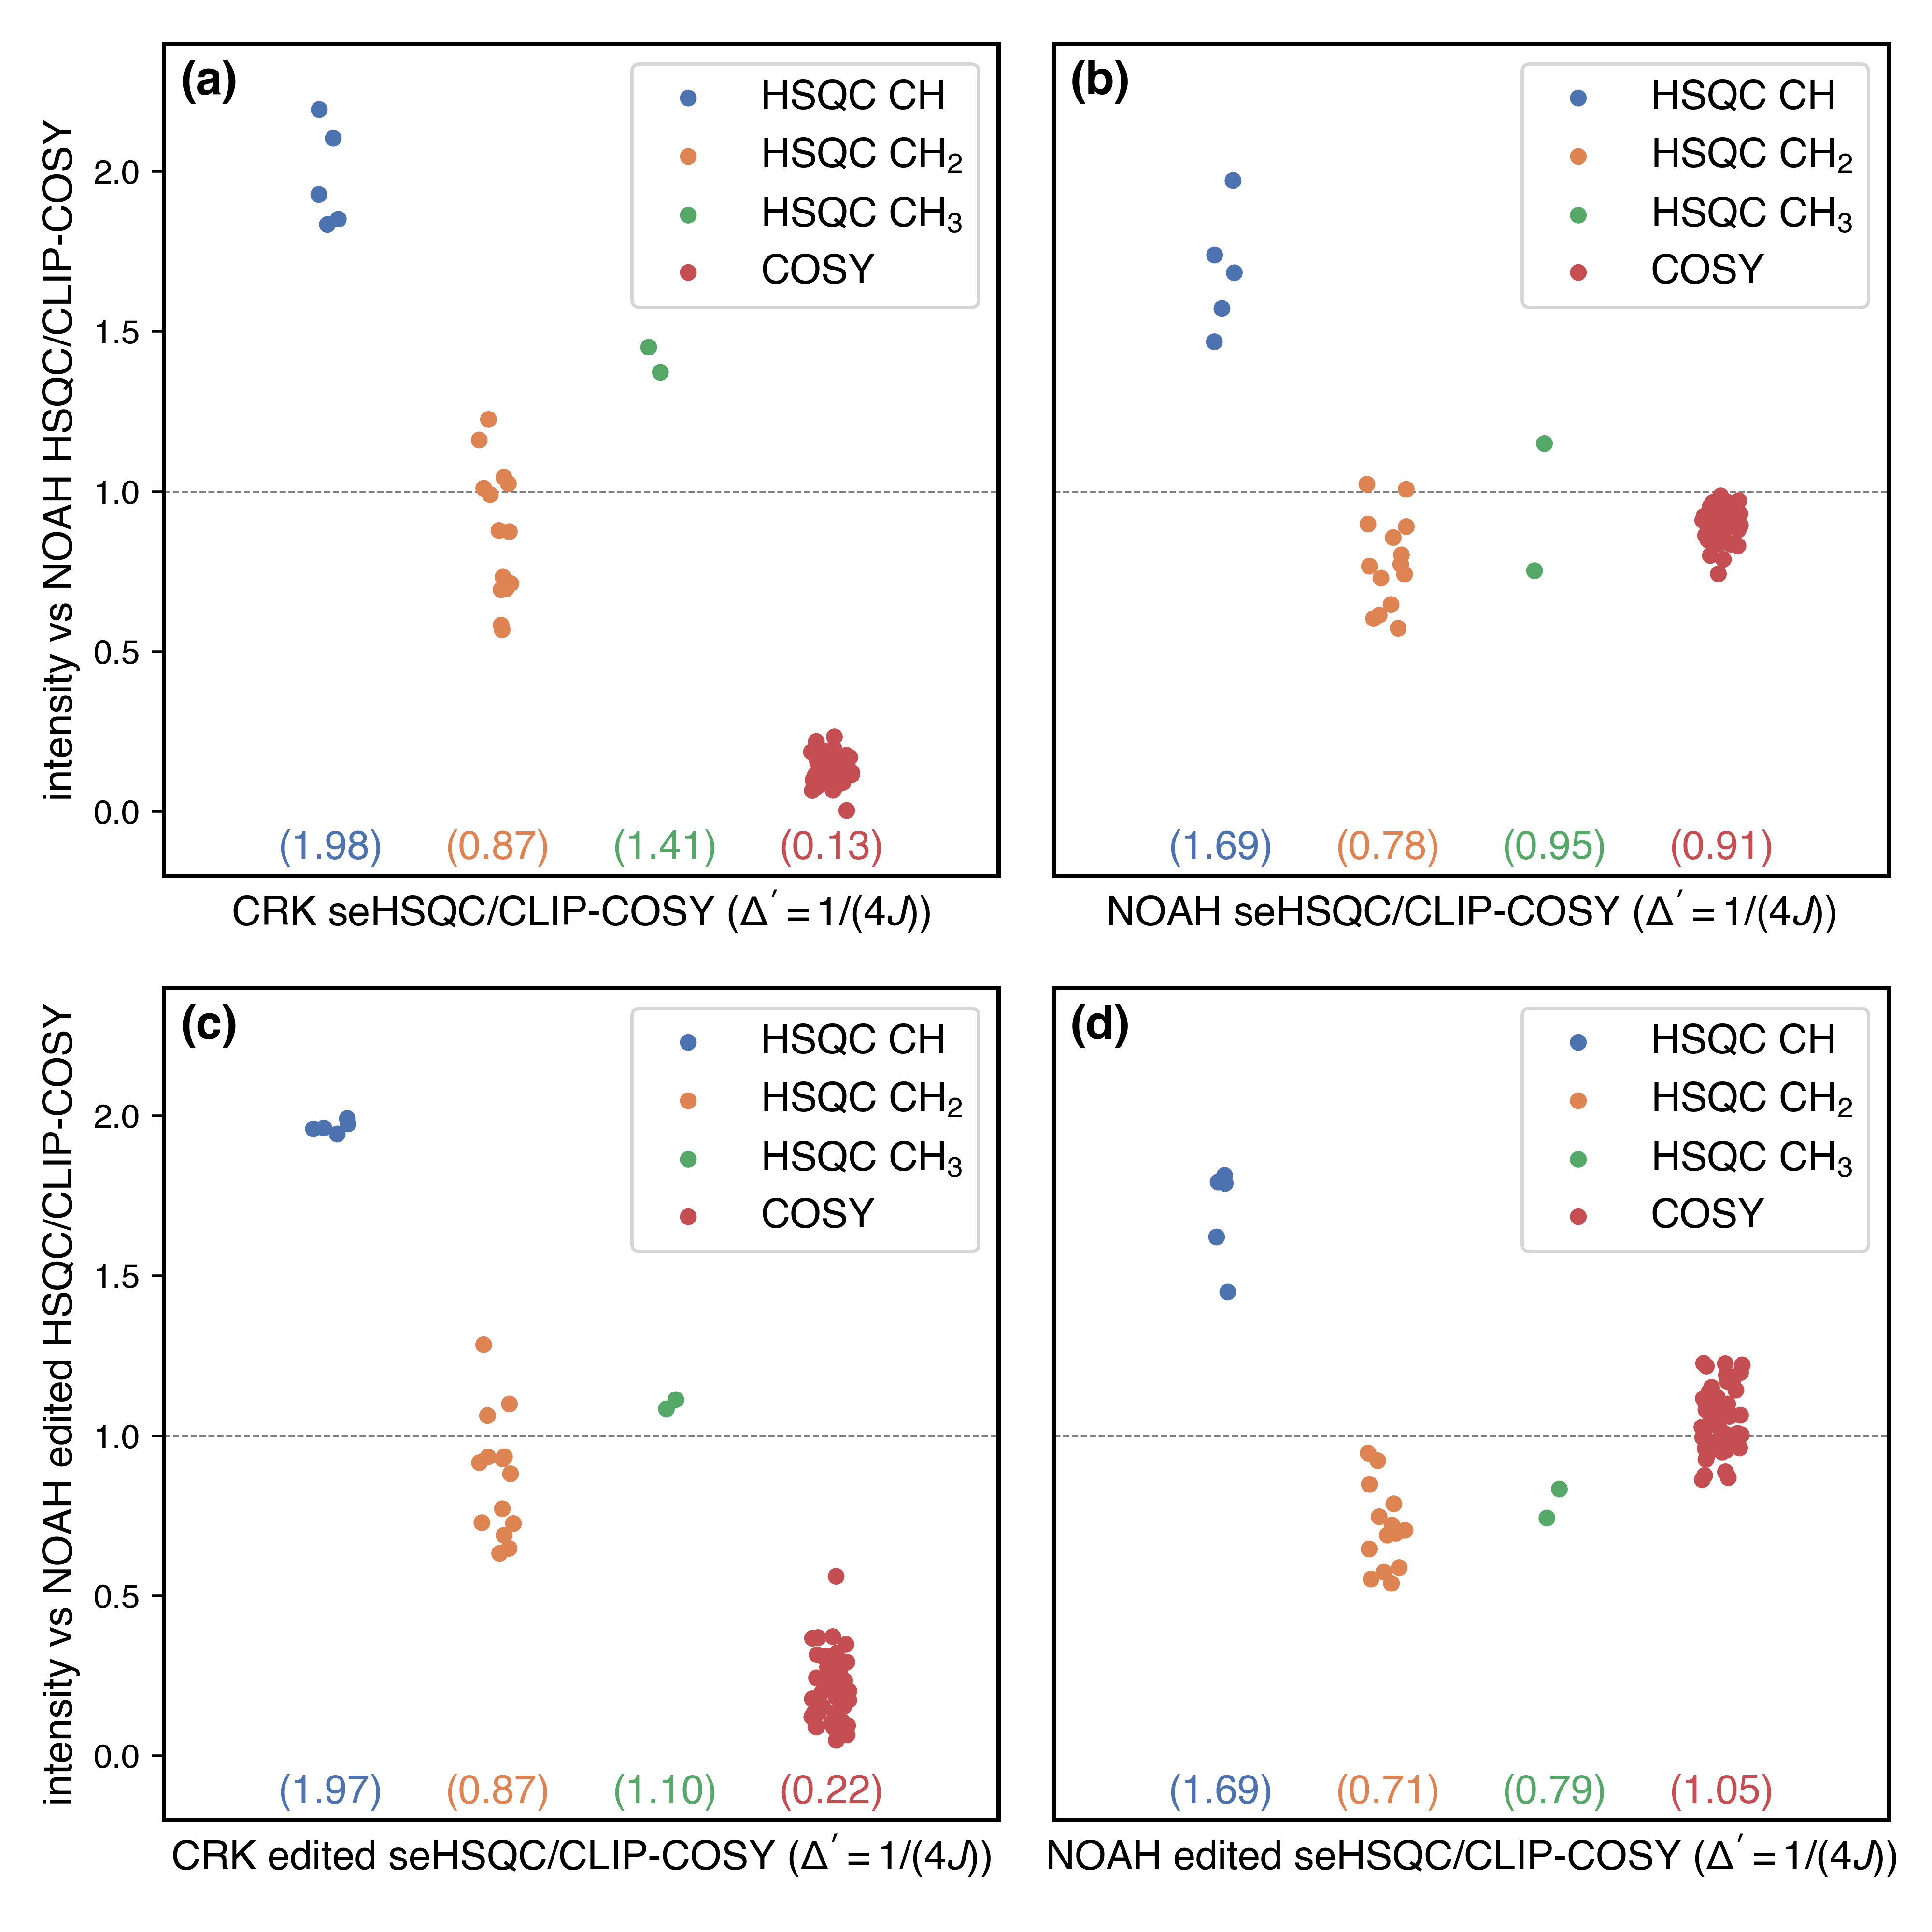
\includegraphics[width=0.8\textwidth]{./figures/combined_1_4j.png}
    \caption{
        Sensitivity of seHSQC sequences with $\Delta'$ set to $1/(4\cdot\onejch)$, versus the corresponding NOAH HSQC/CLIP-COSY supersequence (i.e.\ unedited for (a) and (b), edited for (c) and (d)).
        \textbf{(a)} CRK seHSQC + CLIP-COSY, without multiplicity editing.
        \textbf{(b)} NOAH seHSQC + CLIP-COSY, without multiplicity editing.
        \textbf{(c)} CRK seHSQC + CLIP-COSY, with multiplicity editing.
        \textbf{(d)} NOAH seHSQC + CLIP-COSY, with multiplicity editing.
        \andro{}
    }
    \label{fig:combined_1_4j}
\end{figure}

In particular, for the NOAH seHSQC, we note that the improvements in HSQC \ce{CH} sensitivity gained by moving from $\Delta' = 1/(8\cdot\onejch)$ to $\Delta' = 1/(4\cdot\onejch)$ are marginal (ca.\ 10\%).
At the same time, sensitivity \textit{losses} are observed for \ce{CH2} and \ce{CH3} peaks, likely due to pulse imperfections.

\section{Comparison of BIG-BIRD and ISR elements}

The BIG-BIRD element used here was ${45^\circ}_{45^\circ}(\proton{}) - 2\Delta - 180^\circ(\proton{},\carbon{}) - 2\Delta - {45^\circ}_{225^\circ}(\proton{})$ for the unedited NOAH seHSQC, where $\beta_\phi$ indicates a hard pulse with flip angle $\beta$ and phase $\phi$, and $\Delta = 1/(4\cdot\onejch)$.
For the edited NOAH seHSQC, the BIG-BIRD pulse phases are slightly modified to give ${45^\circ}_{315^\circ}(\proton{}) - 2\Delta - 180^\circ(\proton{},\carbon{}) - 2\Delta - {45^\circ}_{135^\circ}(\proton{})$.
These, and the ISR, have the same net effect on coupled and uncoupled proton magnetisation, as shown in \figref{pprogs_prodop}.
However, the ISR provides greater sensitivity in both the HSQC and downstream COSY.

\begin{figure}
    \centering
    % figures/bigbird.py
    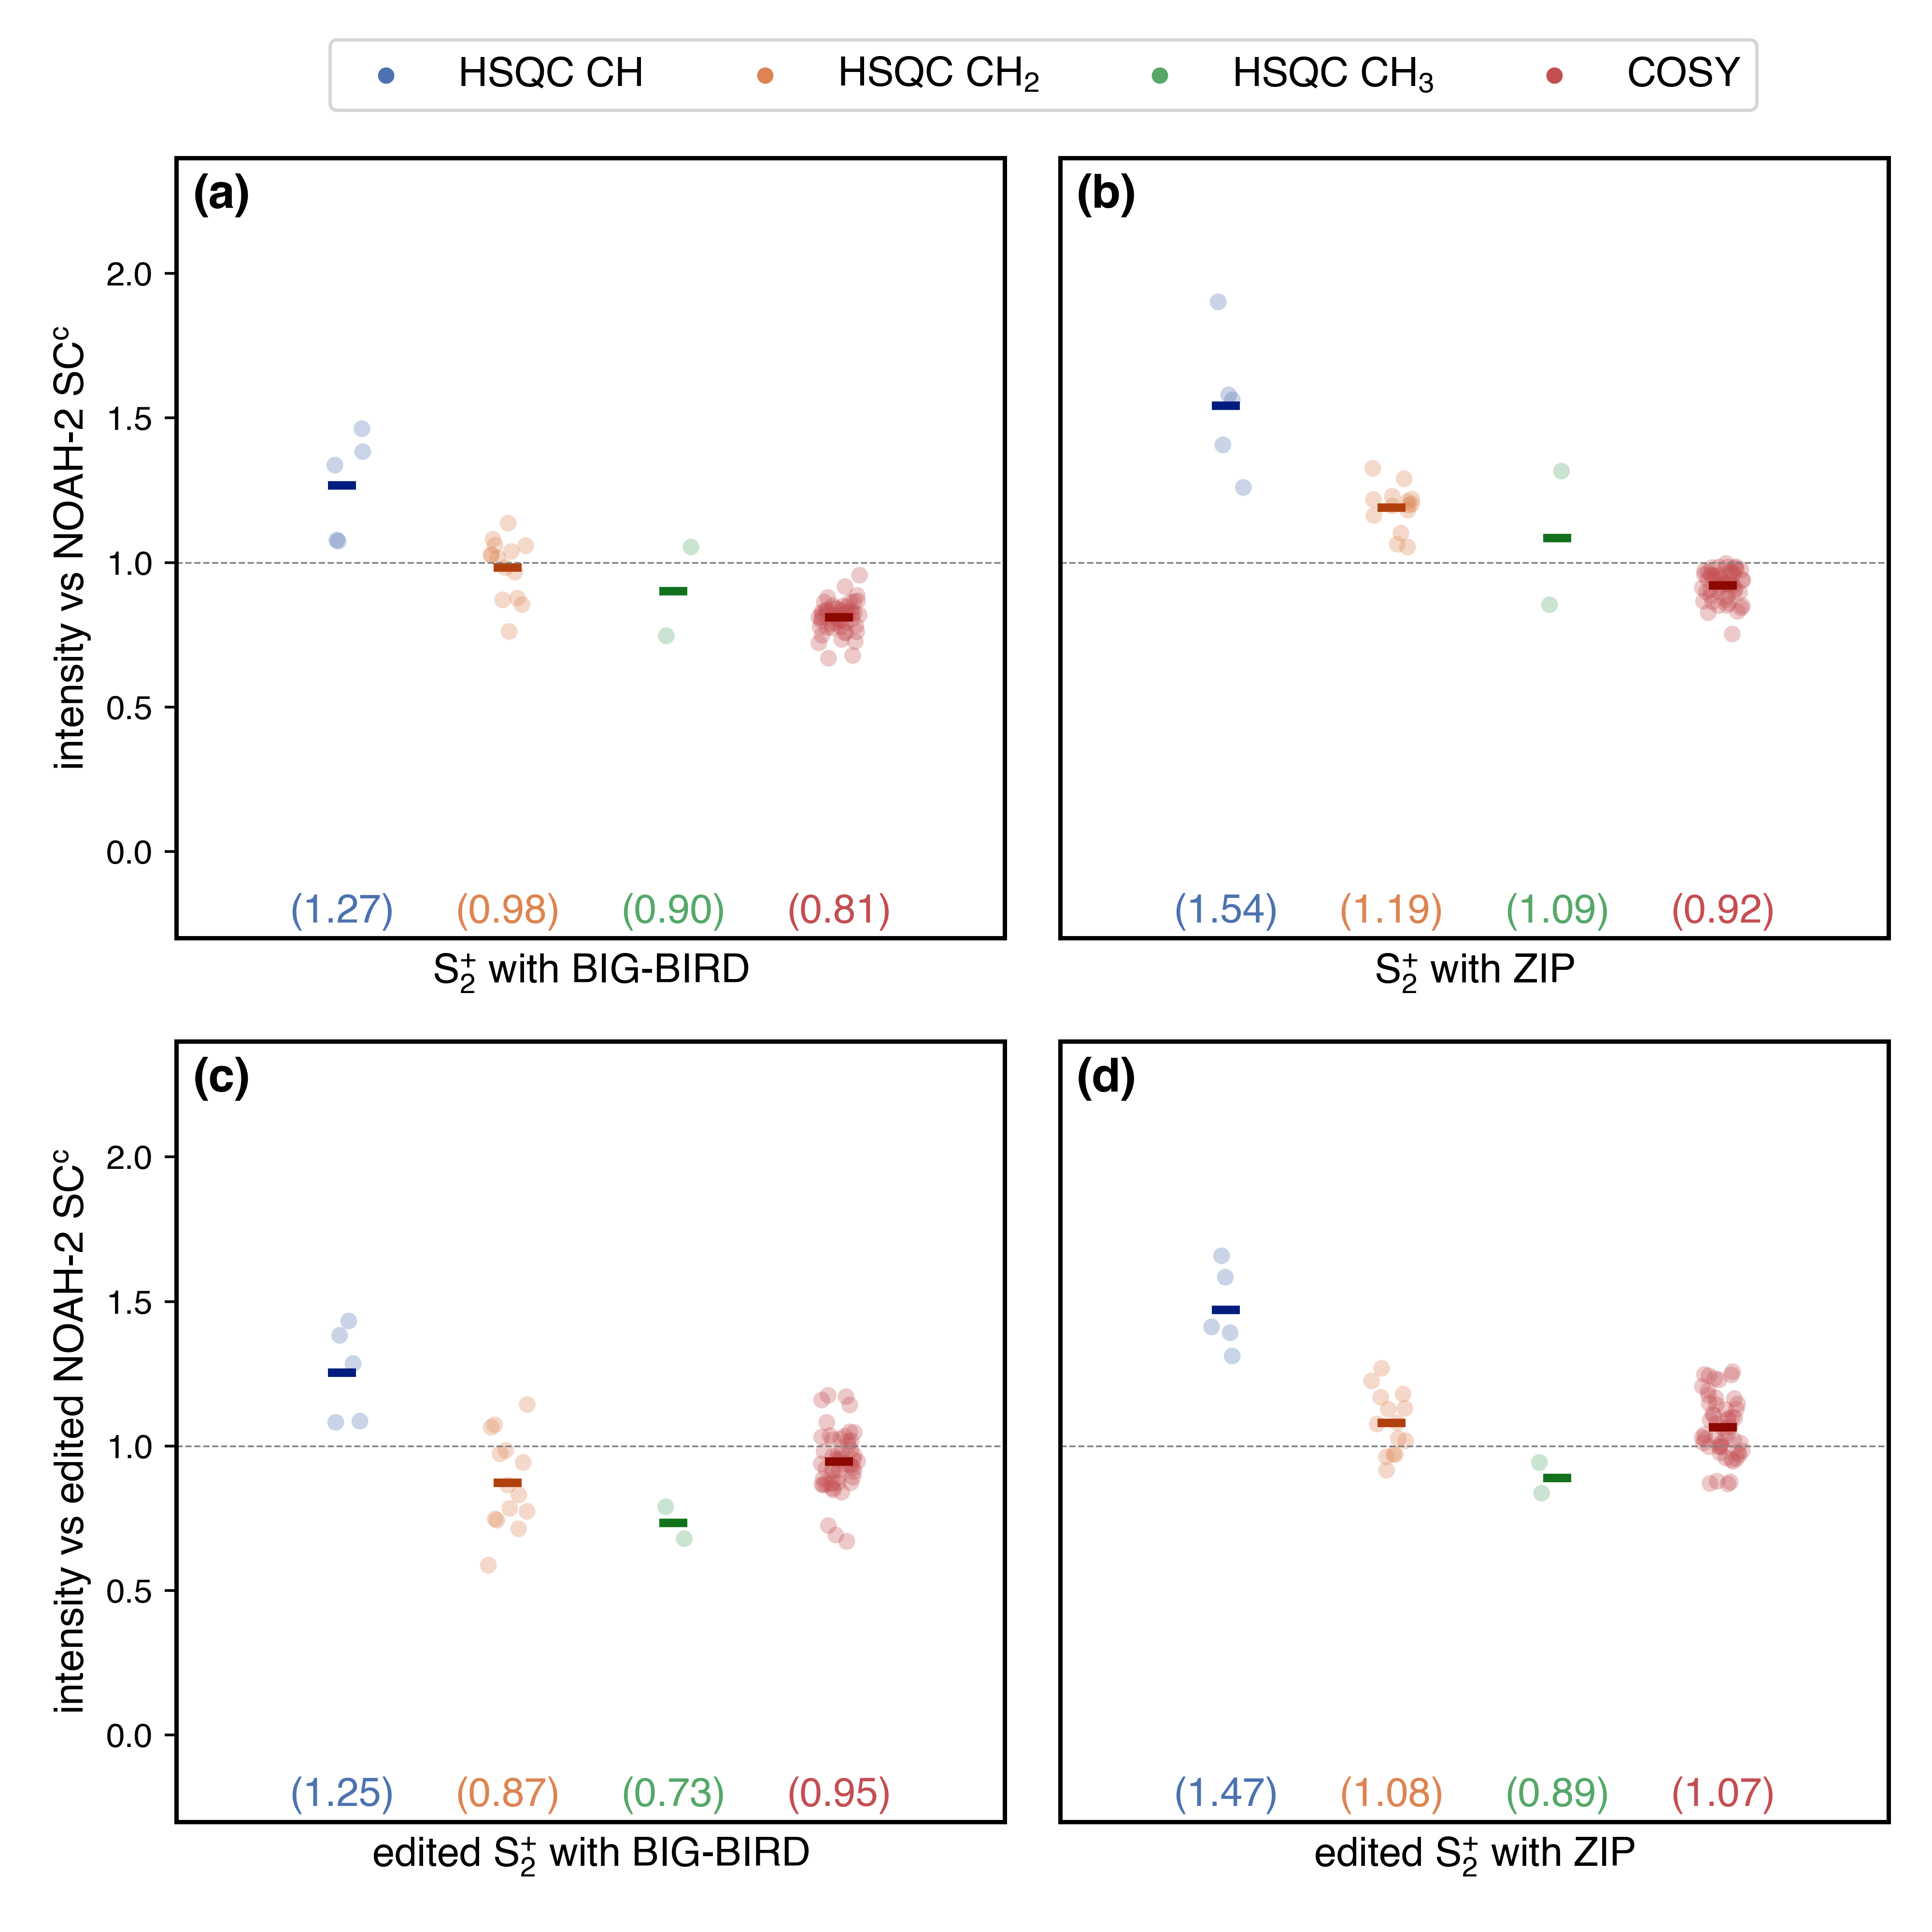
\includegraphics[width=0.8\textwidth]{./figures/bigbird.png}
    \caption{
        Sensitivity of NOAH seHSQC sequences with prepended BIG-BIRD and ISR elements, versus the corresponding NOAH HSQC/CLIP-COSY supersequence (i.e.\ unedited for (a) and (b), edited for (c) and (d)).
        \textbf{(a)} NOAH seHSQC with BIG-BIRD + CLIP-COSY, without multiplicity editing.
        \textbf{(b)} NOAH seHSQC with ISR + CLIP-COSY, without multiplicity editing.
        \textbf{(c)} NOAH seHSQC with BIG-BIRD + CLIP-COSY, with multiplicity editing.
        \textbf{(d)} NOAH seHSQC with ISR + CLIP-COSY, with multiplicity editing.
        \andro{}
    }
    \label{fig:bigbird}
\end{figure}


\section{Suppression of wing artefacts}

The origin of the ``wing'' artefacts in the final homonuclear modules can be most clearly seen from the following series of experiments involving the NOAH-3 \nitrogen{} seHSQC/\carbon{} seHSQC/CLIP-COSY (SpnSpCc) supersequence.
Since the $f_1$ spectral windows of the two seHSQC modules are different, they lead to distinct sets of wing artefacts if the extra gradient before $t_1$ is not present.
\figref{wing_artefacts} focuses on the artefacts associated with intense methyl group peaks, but similar artefacts are observed for all other peaks, albeit with lower absolute intensities.

\begin{figure}
    \centering
    % figures/wing_artefacts.py
    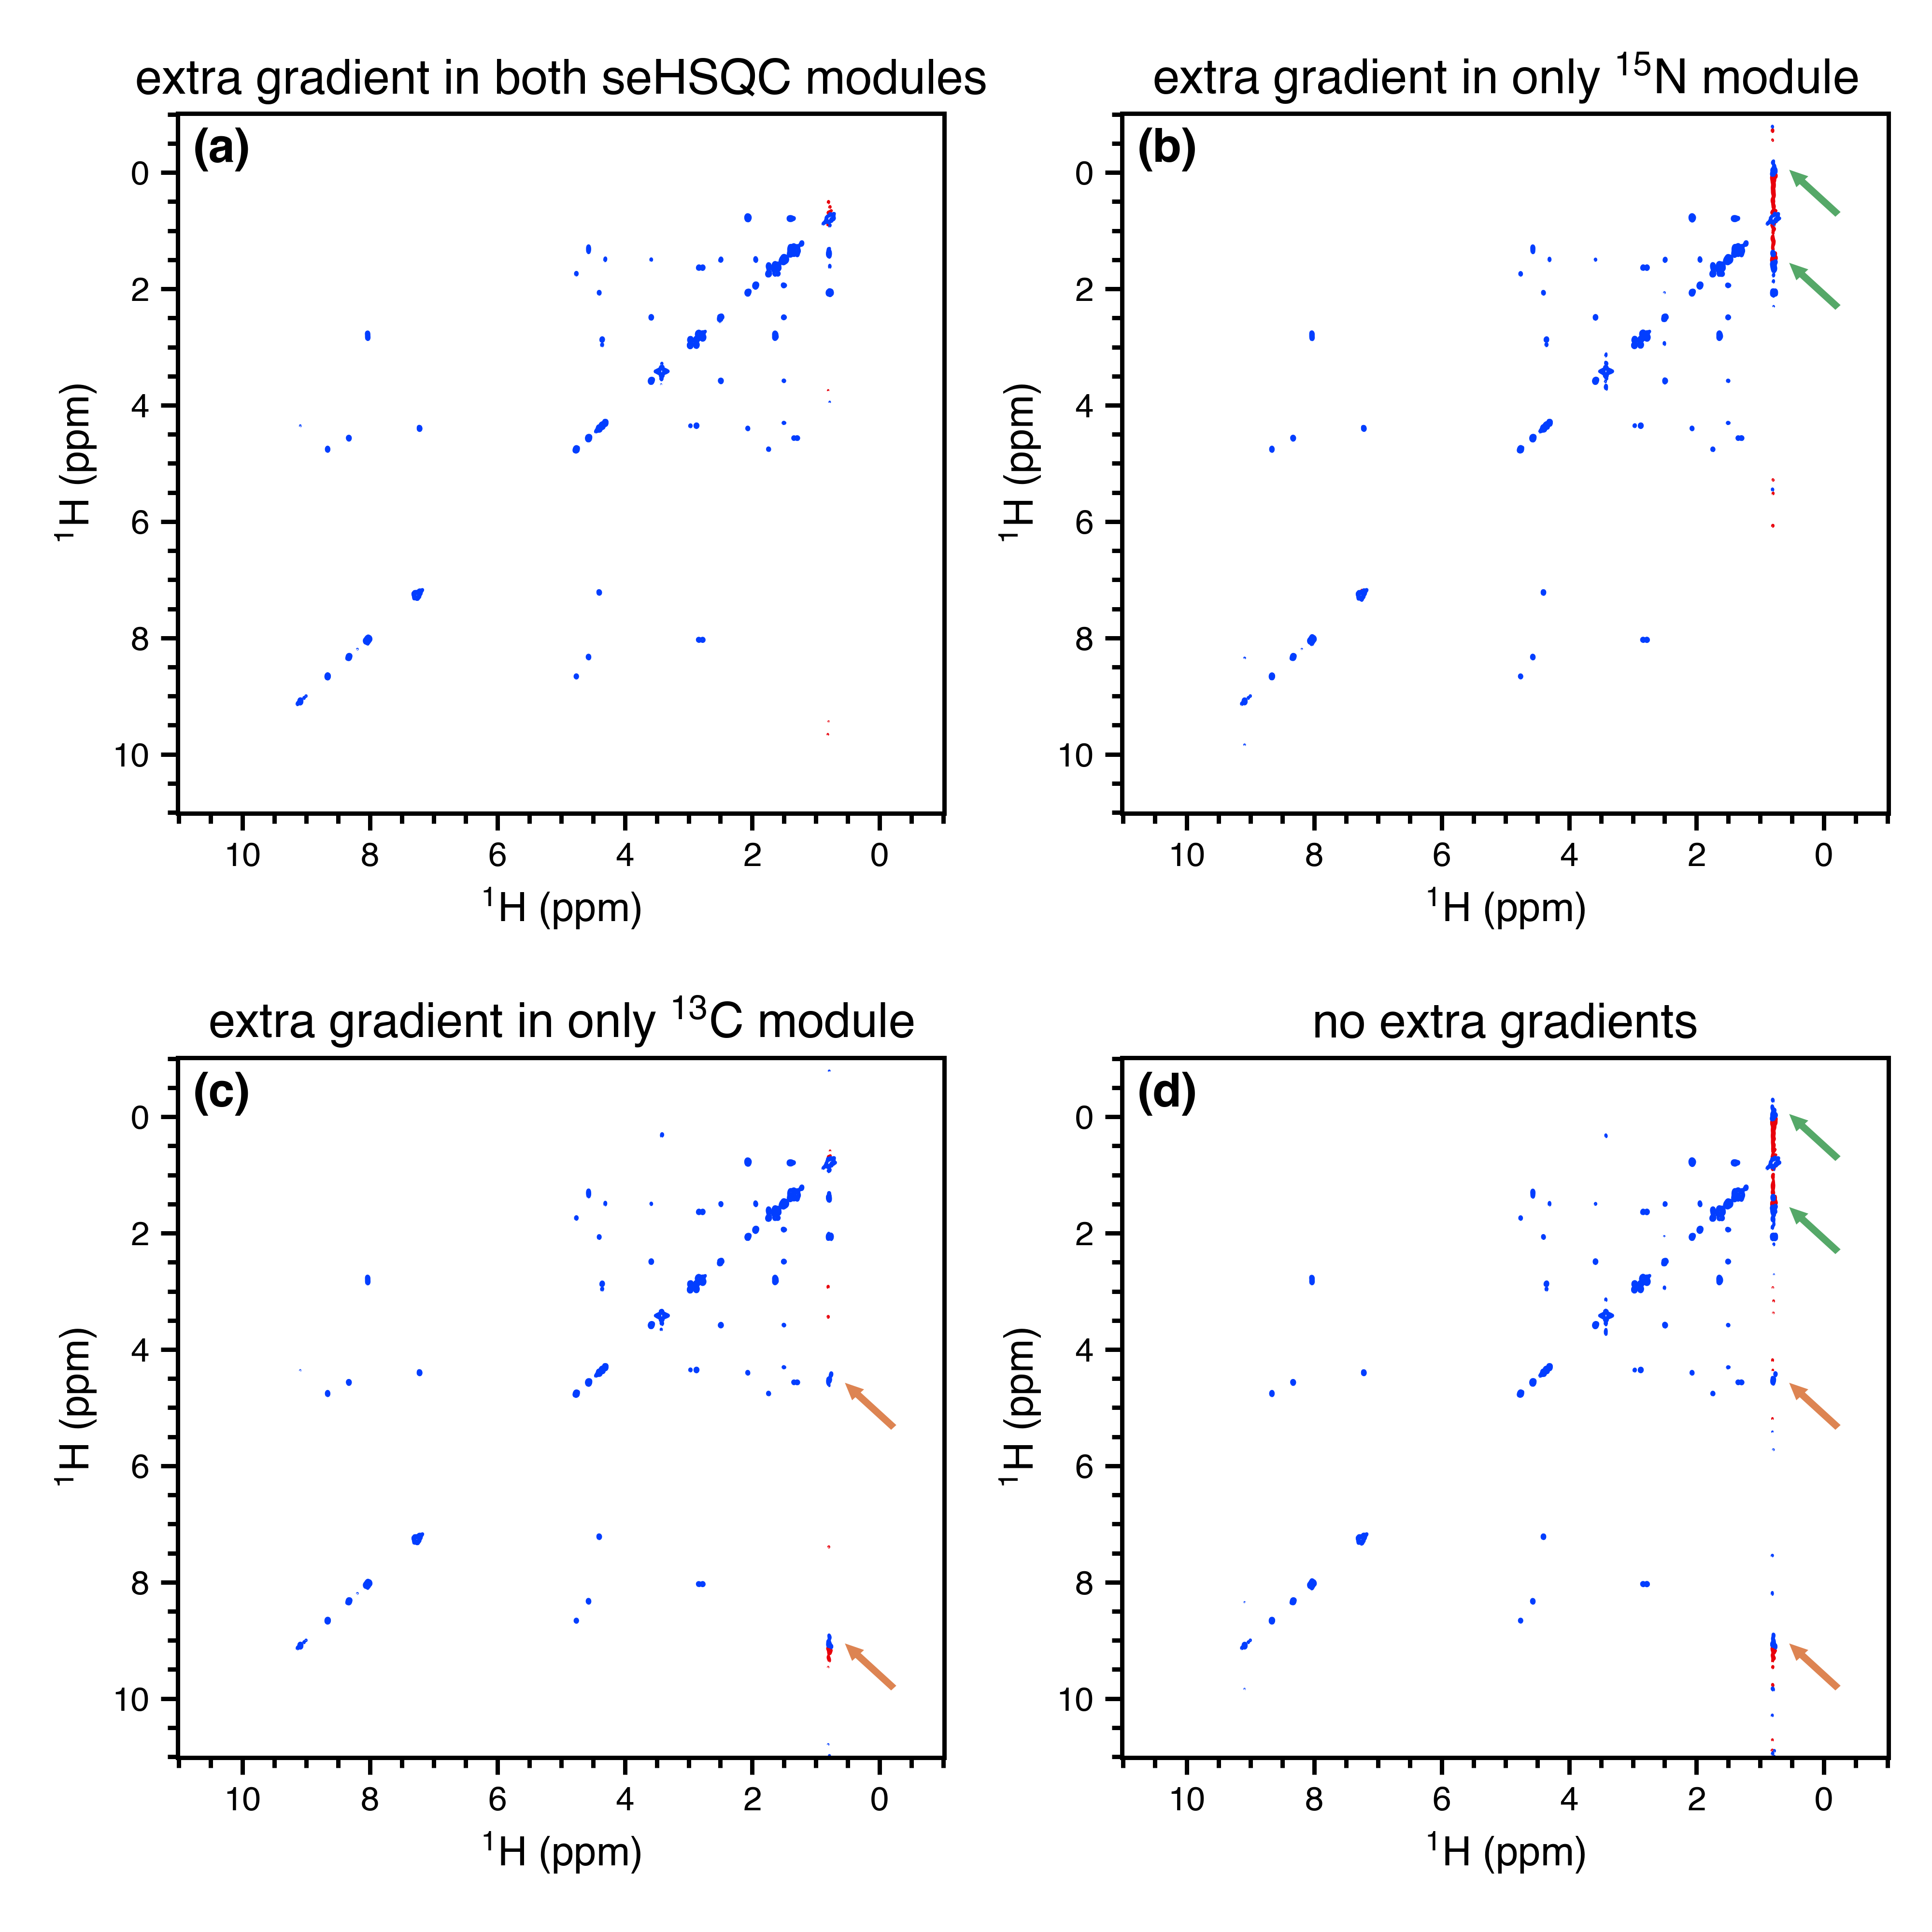
\includegraphics[width=0.8\textwidth]{./figures/wing_artefacts.png}
    \caption{
        CLIP-COSY spectra obtained from various forms of the NOAH-3 SpnSpCc supersequence.
        Wing artefacts arising from the \nitrogen{} seHSQC are highlighted in orange; those arising from the \carbon{} seHSQC in green.
        Notice how (in this case) the former can easily be misinterpreted as a crosspeak, while the latter obscures genuine crosspeaks.
        \textbf{(a)} With the extra gradient inserted for both modules, i.e.\ no artefacts.
        \textbf{(b)} With an extra gradient in only the \nitrogen{} module, i.e.\ only the \carbon{} artefacts.
        \textbf{(c)} With an extra gradient in only the \carbon{} module.
        \textbf{(d)} With no extra gradients.
        \grami{}
    }
    \label{fig:wing_artefacts}
\end{figure}


\section{\texorpdfstring{\nitrogen{}}{15N} HSQC and line broadening}

For \nitrogen{}--\proton{} correlations, both the HMQC and the new seHSQC module are recommended as they keep the bulk magnetisation along $\pm z$ during the $t_1$ period.
The HSQC module places bulk magnetisation in the $xy$-plane, leading to $\jhh$ evolution; consequently, the amount of bulk magnetisation ``passed on'' to the downstream modules decreases as the \nitrogen{} $t_1$ is increased.
Since $t_1$ for each NOAH module is incremented in sync, this is manifested in downstream modules as a $t_1$-dependent decrease in amplitude, or $f_1$ line broadening after Fourier transformation, as shown in \figref{n15_linebroadening}.

\begin{figure}
    \centering
    % figures/n15_linebroadening.py
    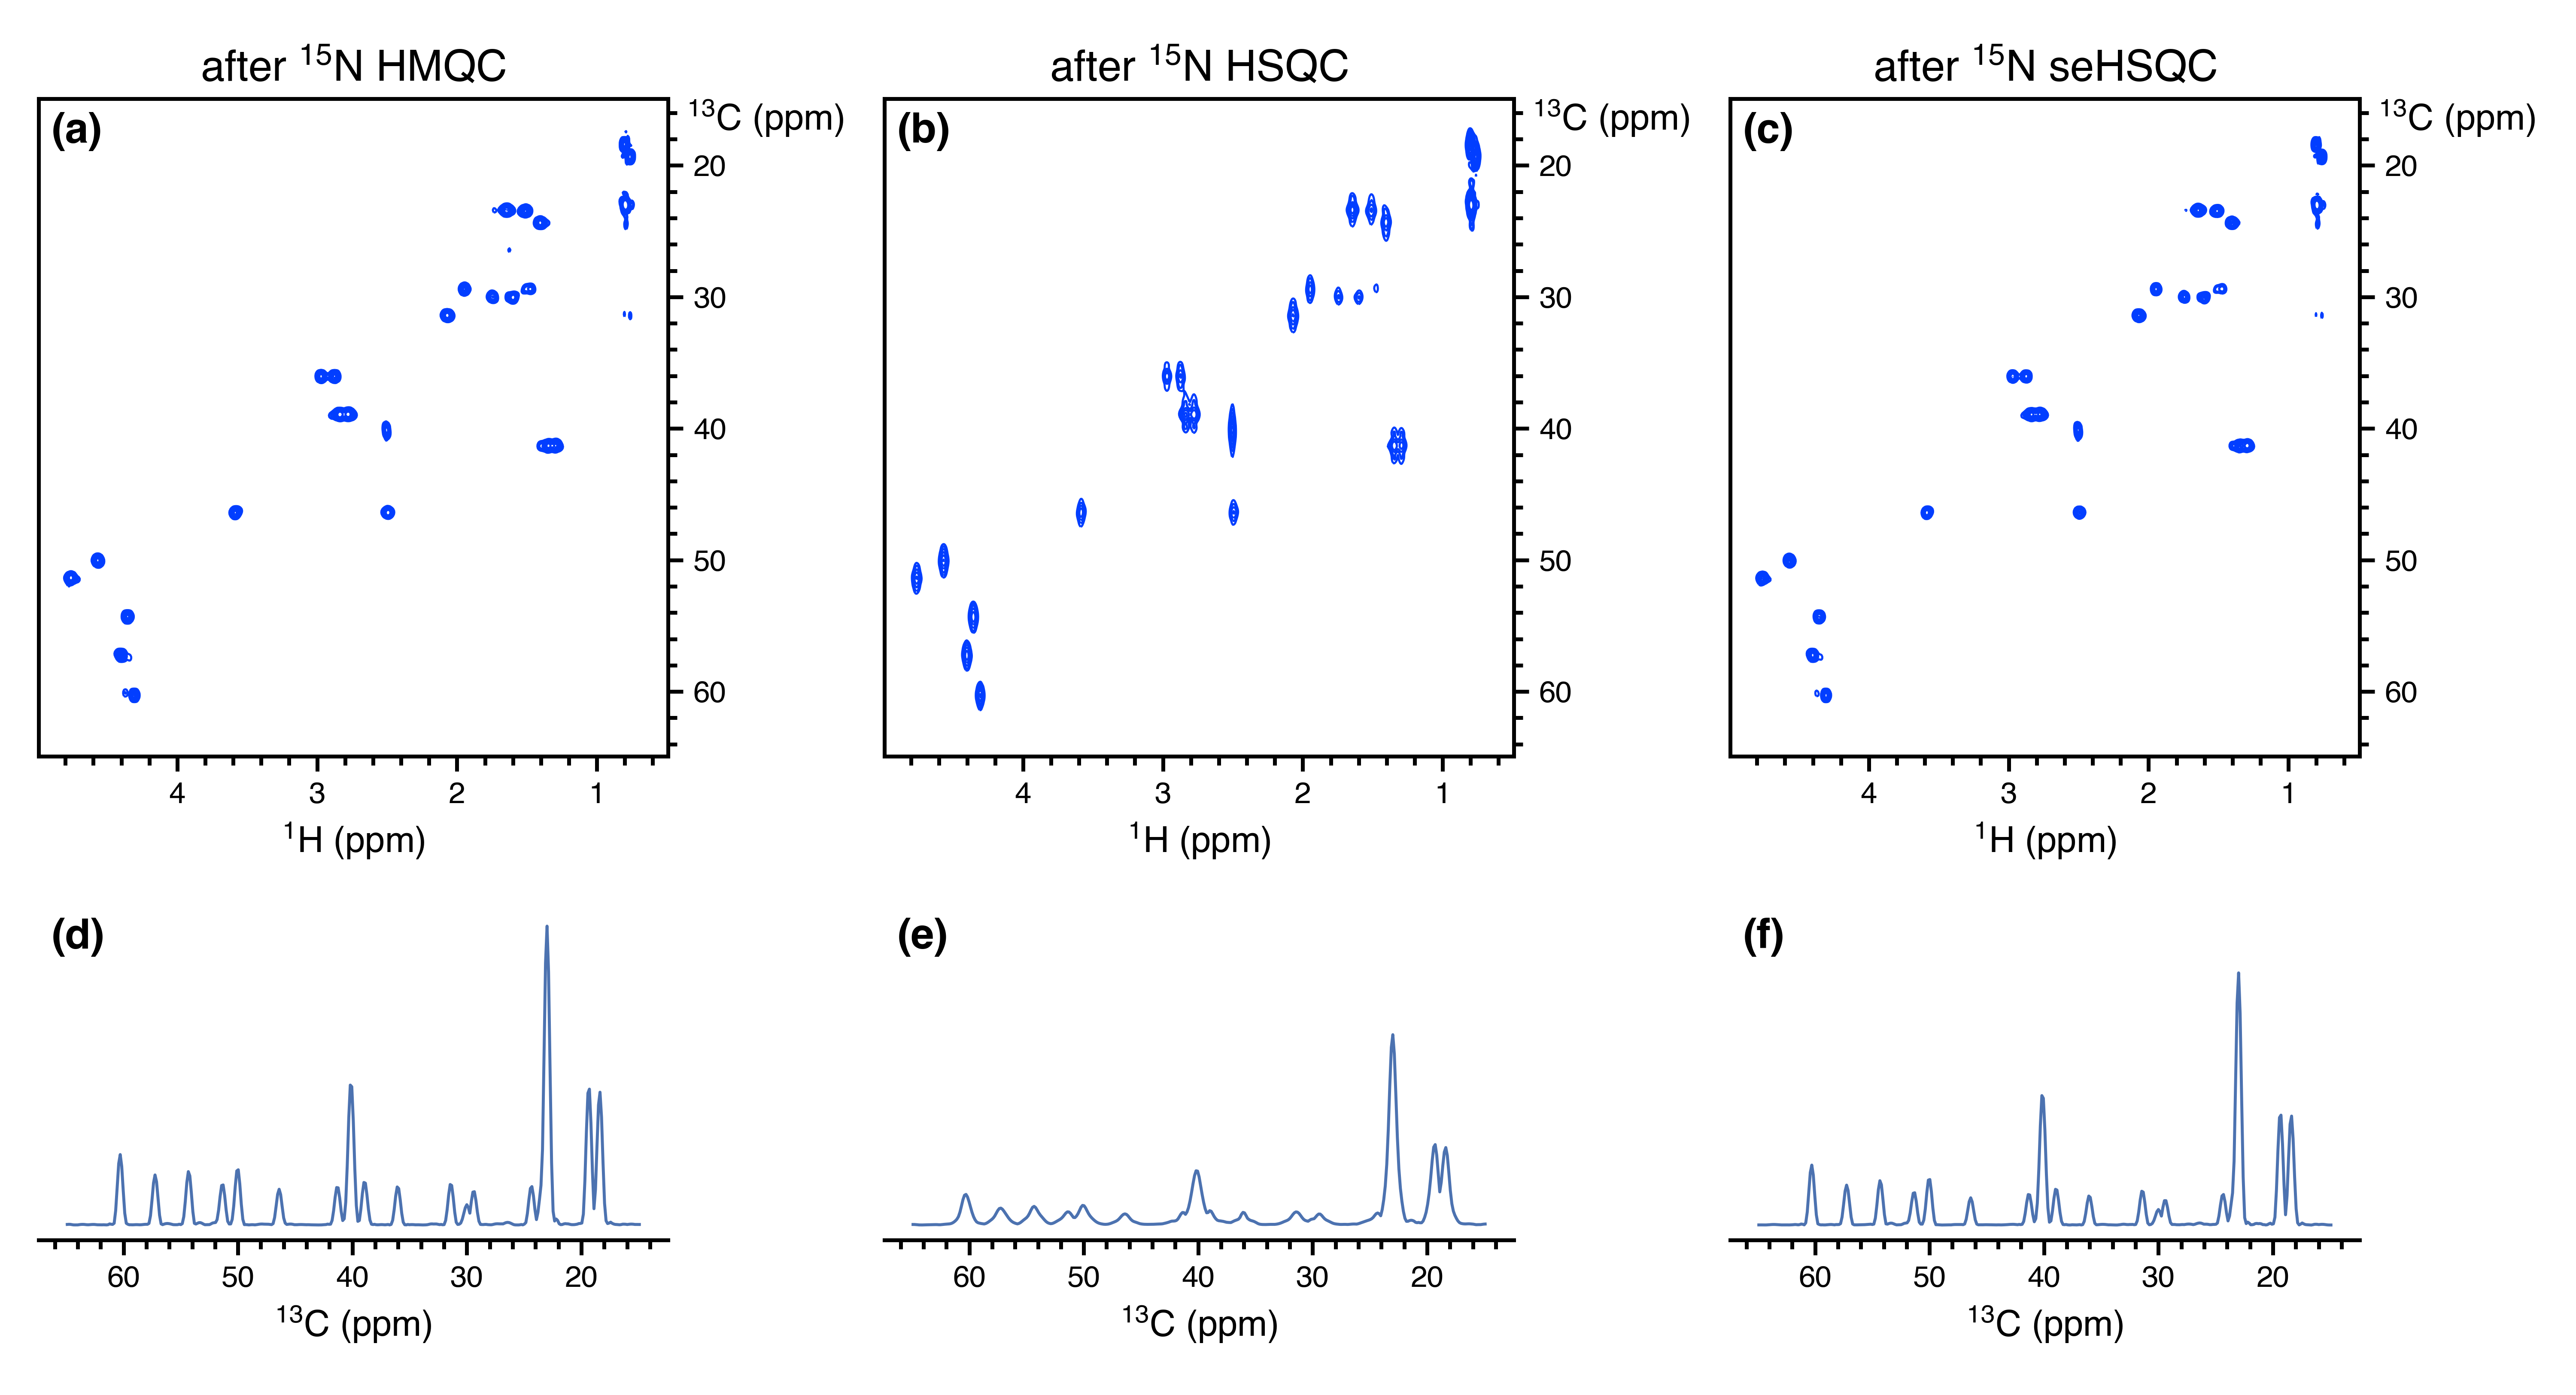
\includegraphics[width=\textwidth]{./figures/n15_linebroadening.png}
    \caption{
        \carbon{} seHSQC spectra obtained from NOAH-3 XSpCc (\nitrogen{} module + \carbon{} seHSQC + CLIP-COSY) supersequences.
        The \nitrogen{} spectral window was \SI{30}{ppm} and 256 $t_1$ increments were collected, corresponding to an indirect-dimension \nitrogen{} acquisition time of \SI{60.1}{\ms}.
        \textbf{(a)} X = HMQC.
        \textbf{(b)} X = HSQC.
        \textbf{(c)} X = seHSQC.
        \textbf{(d)}--\textbf{(f)} Projections of spectra \textbf{(a)}--\textbf{(c)} onto the $f_1$ axis.
        Note the $f_1$ line broadening in (b) and (e).
        \grami{}
    }
    \label{fig:n15_linebroadening}
\end{figure}

This line broadening also leads to a substantial sensitivity loss (almost 65\% in \figref{n15_linebroadening}).
The extent of the line broadening depends on the acquisition time, and is particularly pronounced for long acquisition times, i.e.\ small \nitrogen{} spectral windows.
In our experience, at \nitrogen{} acquisition times of ca.\ \SI{5}{\ms} the effect is almost indiscernible.
Such a short acquisition time would lead to poor resolution in the \nitrogen{} dimension itself, which may or may not be tolerable.
Of course, this issue can be entirely avoided by using either the HMQC or seHSQC.

\section{Effect of lengthened gradients in \texorpdfstring{\nitrogen{}}{15N} experiments}

\begin{figure}
    \centering
    % figures/cnst16_diff.py
    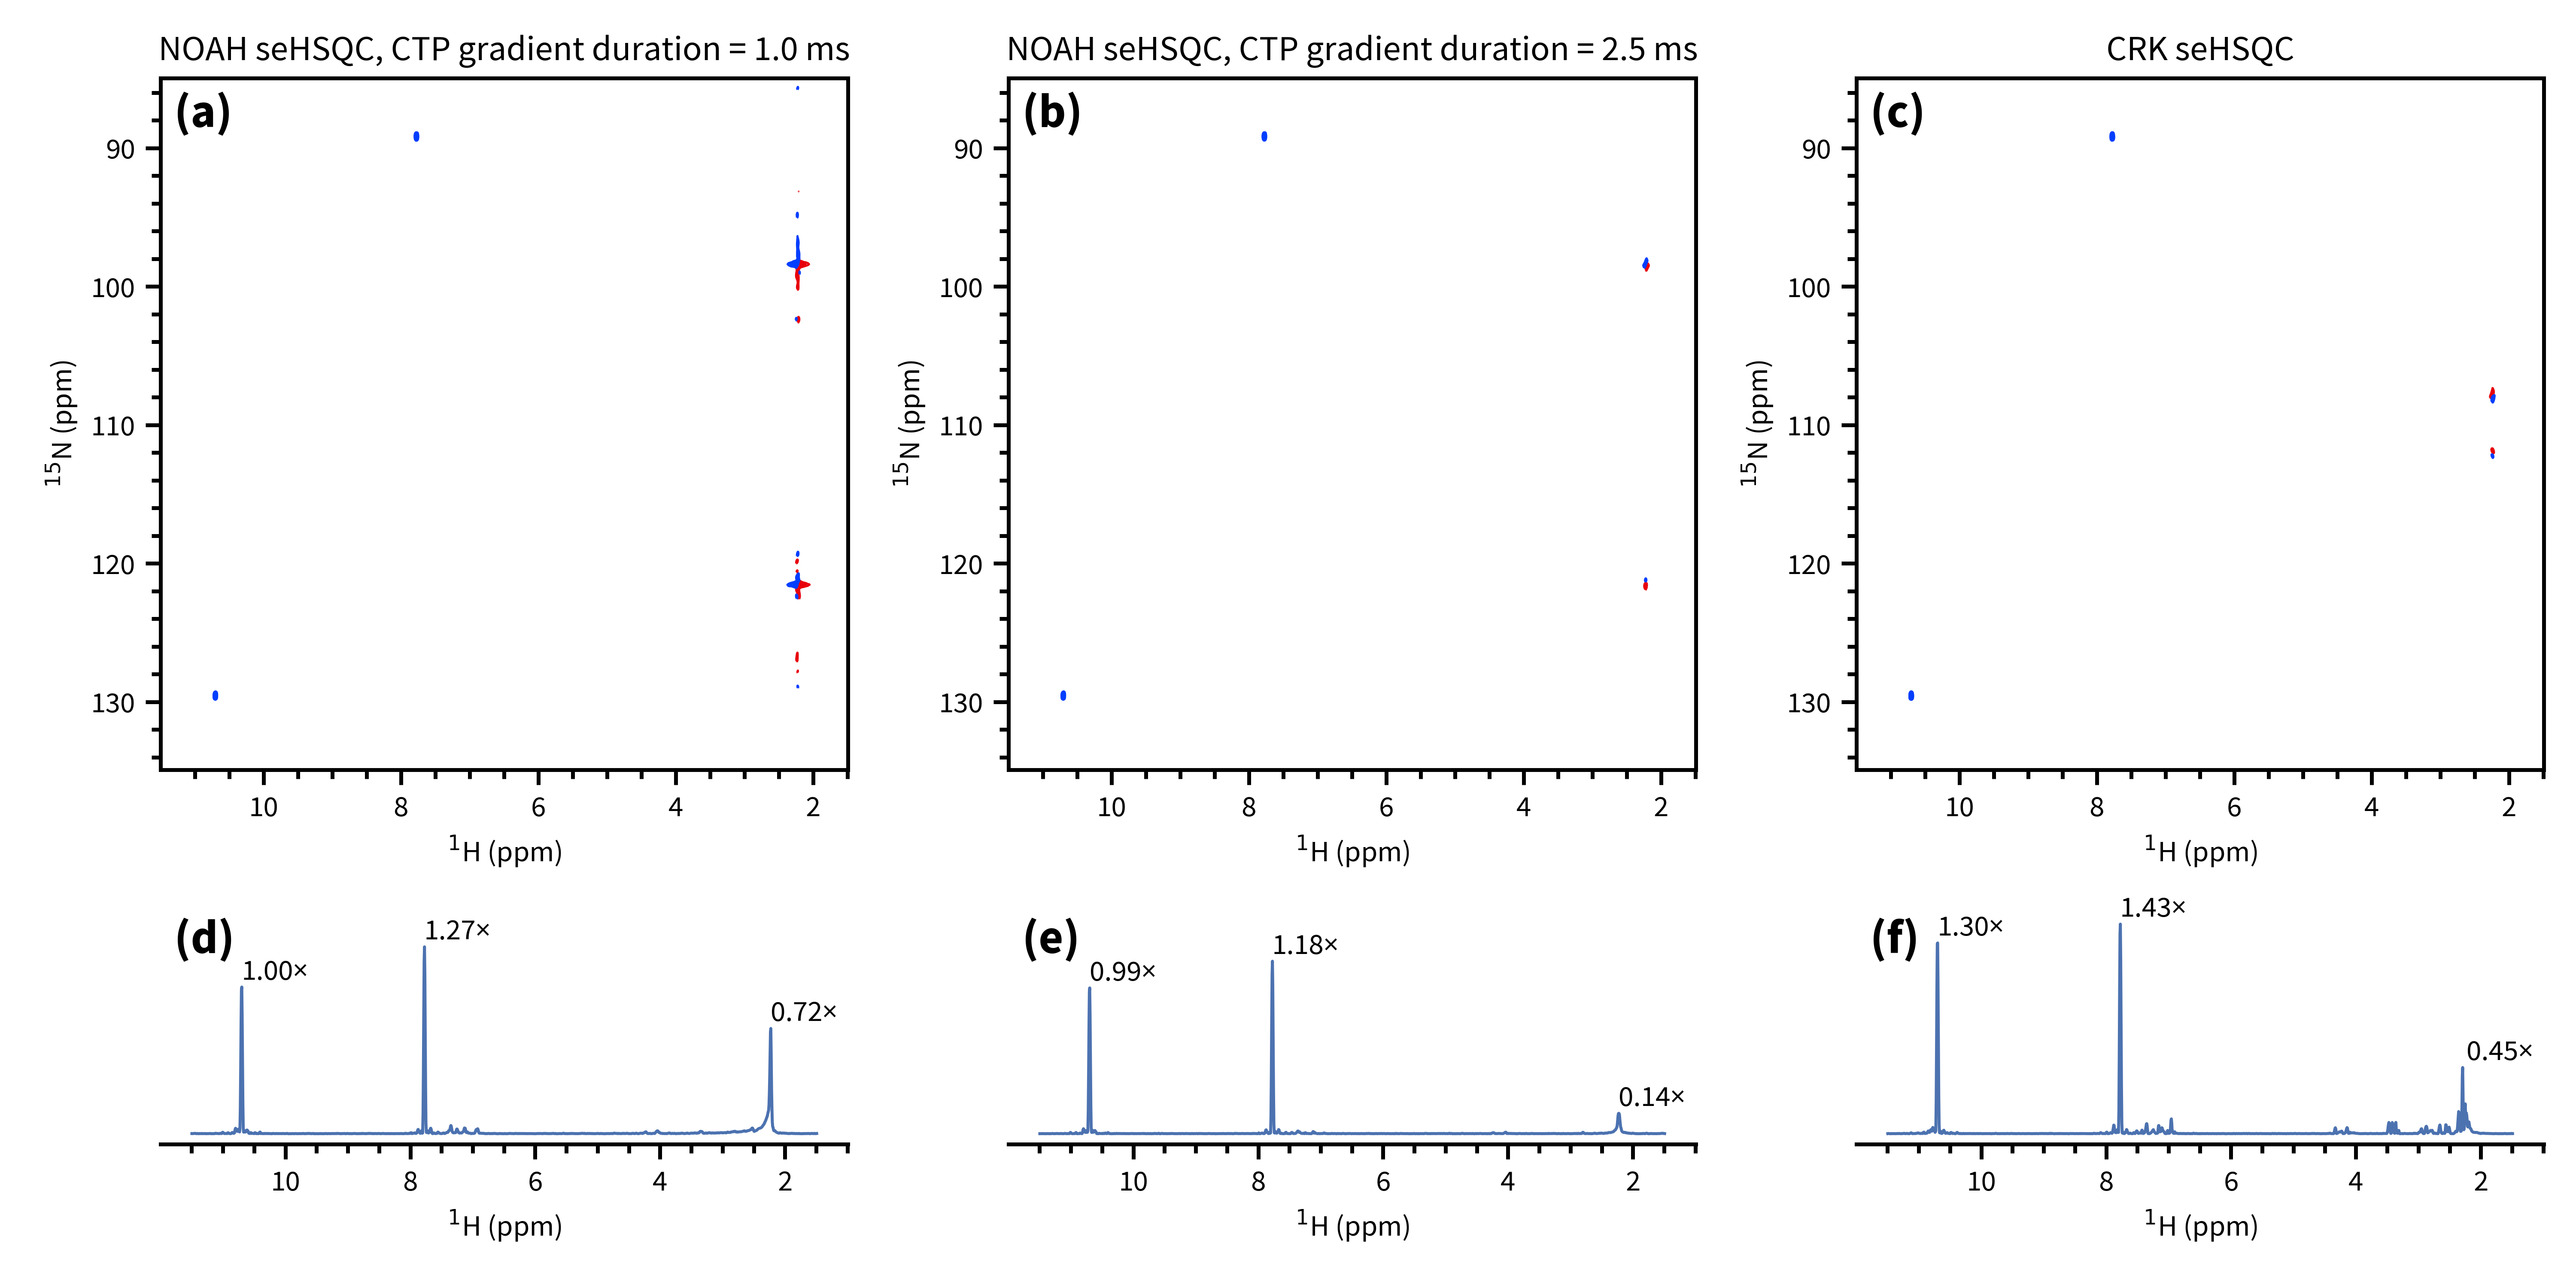
\includegraphics[width=\textwidth]{./figures/cnst16_diff.png}
    \caption{
        \nitrogen{} seHSQC spectra obtained using the NOAH and CRK implementations.
        The peaks at 7.8 and \SI{10.7}{\ppm} (\proton{} shifts) are genuine crosspeaks; the mixed-phase peaks at \SI{2.2}{\ppm} are artefacts.
        \textbf{(a)} NOAH seHSQC, with original CTP gradients of \SI{1}{\ms}.
        \textbf{(b)} NOAH seHSQC, with longer CTP gradients of \SI{1}{\ms}.
        \textbf{(c)} Standalone CRK seHSQC with \SI{1}{\ms} CTP gradients.
        \textbf{(d)}--\textbf{(f)} Projections of spectra \textbf{(a)}--\textbf{(c)} onto the $f_2$ axis.
        The numbers indicate relative peak heights (normalised against the \SI{10.7}{\ppm} peak in (d)).
        \zolmi{}
    }
    \label{fig:cnst16_diff}
\end{figure}

The lengthening of CTP gradients from \SI{1}{\ms} to \SI{2.5}{\ms} is aimed at cleaning up artefacts arising from bulk magnetisation that is not properly returned to $+z$ at the end of the sequence.
\figref{cnst16_diff} shows exactly how effective this strategy is.
In (d), where the CTP gradients have their original duration, the artefacts have comparable intensity to the desired peaks.
When the gradients are lengthened in (e), the crosspeak intensities are almost unaffected (with losses of $<10\%$ arising perhaps from relaxation and diffusion).
However, the artefacts are suppressed by a factor of 5 or more.
Although this suppression is not complete, this should not be interpreted as a weakness of the new NOAH seHSQC module, as similar artefacts are also visible in the CRK seHSQC (f).
Indeed, every \nitrogen{}--\proton{} experiment we tested has at least \textit{some} artefact intensity in this region.

\section{Effect of \texorpdfstring{$k$}{k}-scaling}

The effect of $k$-scaling on the HMQC is shown in \figref{hmqc_kscale}.
By decreasing the indirect dimension resolution, the $f_1$ linewidths of the peaks increase: this can lead to significant sensitivity enhancement for the HMQC (up to $2.7 \times$), because $\jhh$ splitting in the $f_1$ dimension is no longer resolved.
The largest gains are observed for peaks where $\jhh$ splitting is more visible; for the leftmost peak at $\Omega_{\ce{N}} = \SI{128}{\ppm}$, only $1.7 \times$ gains in sensitivity can be attained through this method.

For the seHSQC module, $k$-scaling on its own leads to far smaller sensitivity gains (\figref{spv2_kscale}).
Any increase in the total peak volume is almost completely offset by the $f_1$ broadening.
Therefore, even at $k = 8$, the largest sensitivity gains that can be attained are $\sim 1.3\times$.

The use of linear prediction for spectra with $k > 1$ can, to a certain extent, compensate for the line broadening.
This is less successful for the HMQC spectra (\figref{hmqc_kscale_lp}).
Although raw gains in peak height can be observed for all values of $k$, there is a corresponding decrease in the spectral quality, as evidenced by the $f_1$ multiplet structure being increasingly distorted.
On the other hand, linear prediction performs well for the seHSQC spectra (\figref{spv2_kscale_lp}), where there is no multiplet structure in $f_1$.
Even the reconstruction with $k = 8$ has reasonable spectral quality: although the 2D spectrum (d) appears to have unusual peak shapes, this is merely the result of having the same contour levels as the $k = 1$ spectrum.
The actual peaks are still clearly singlets, as can be seen from the projection in (h).

An additional example of successful $k$-scaling and linear prediction (with $k = 4$) can be seen in Section \ref{section:si_spectra}.

\begin{figure}
    \centering
    % figures/hmqc_kscale.py
    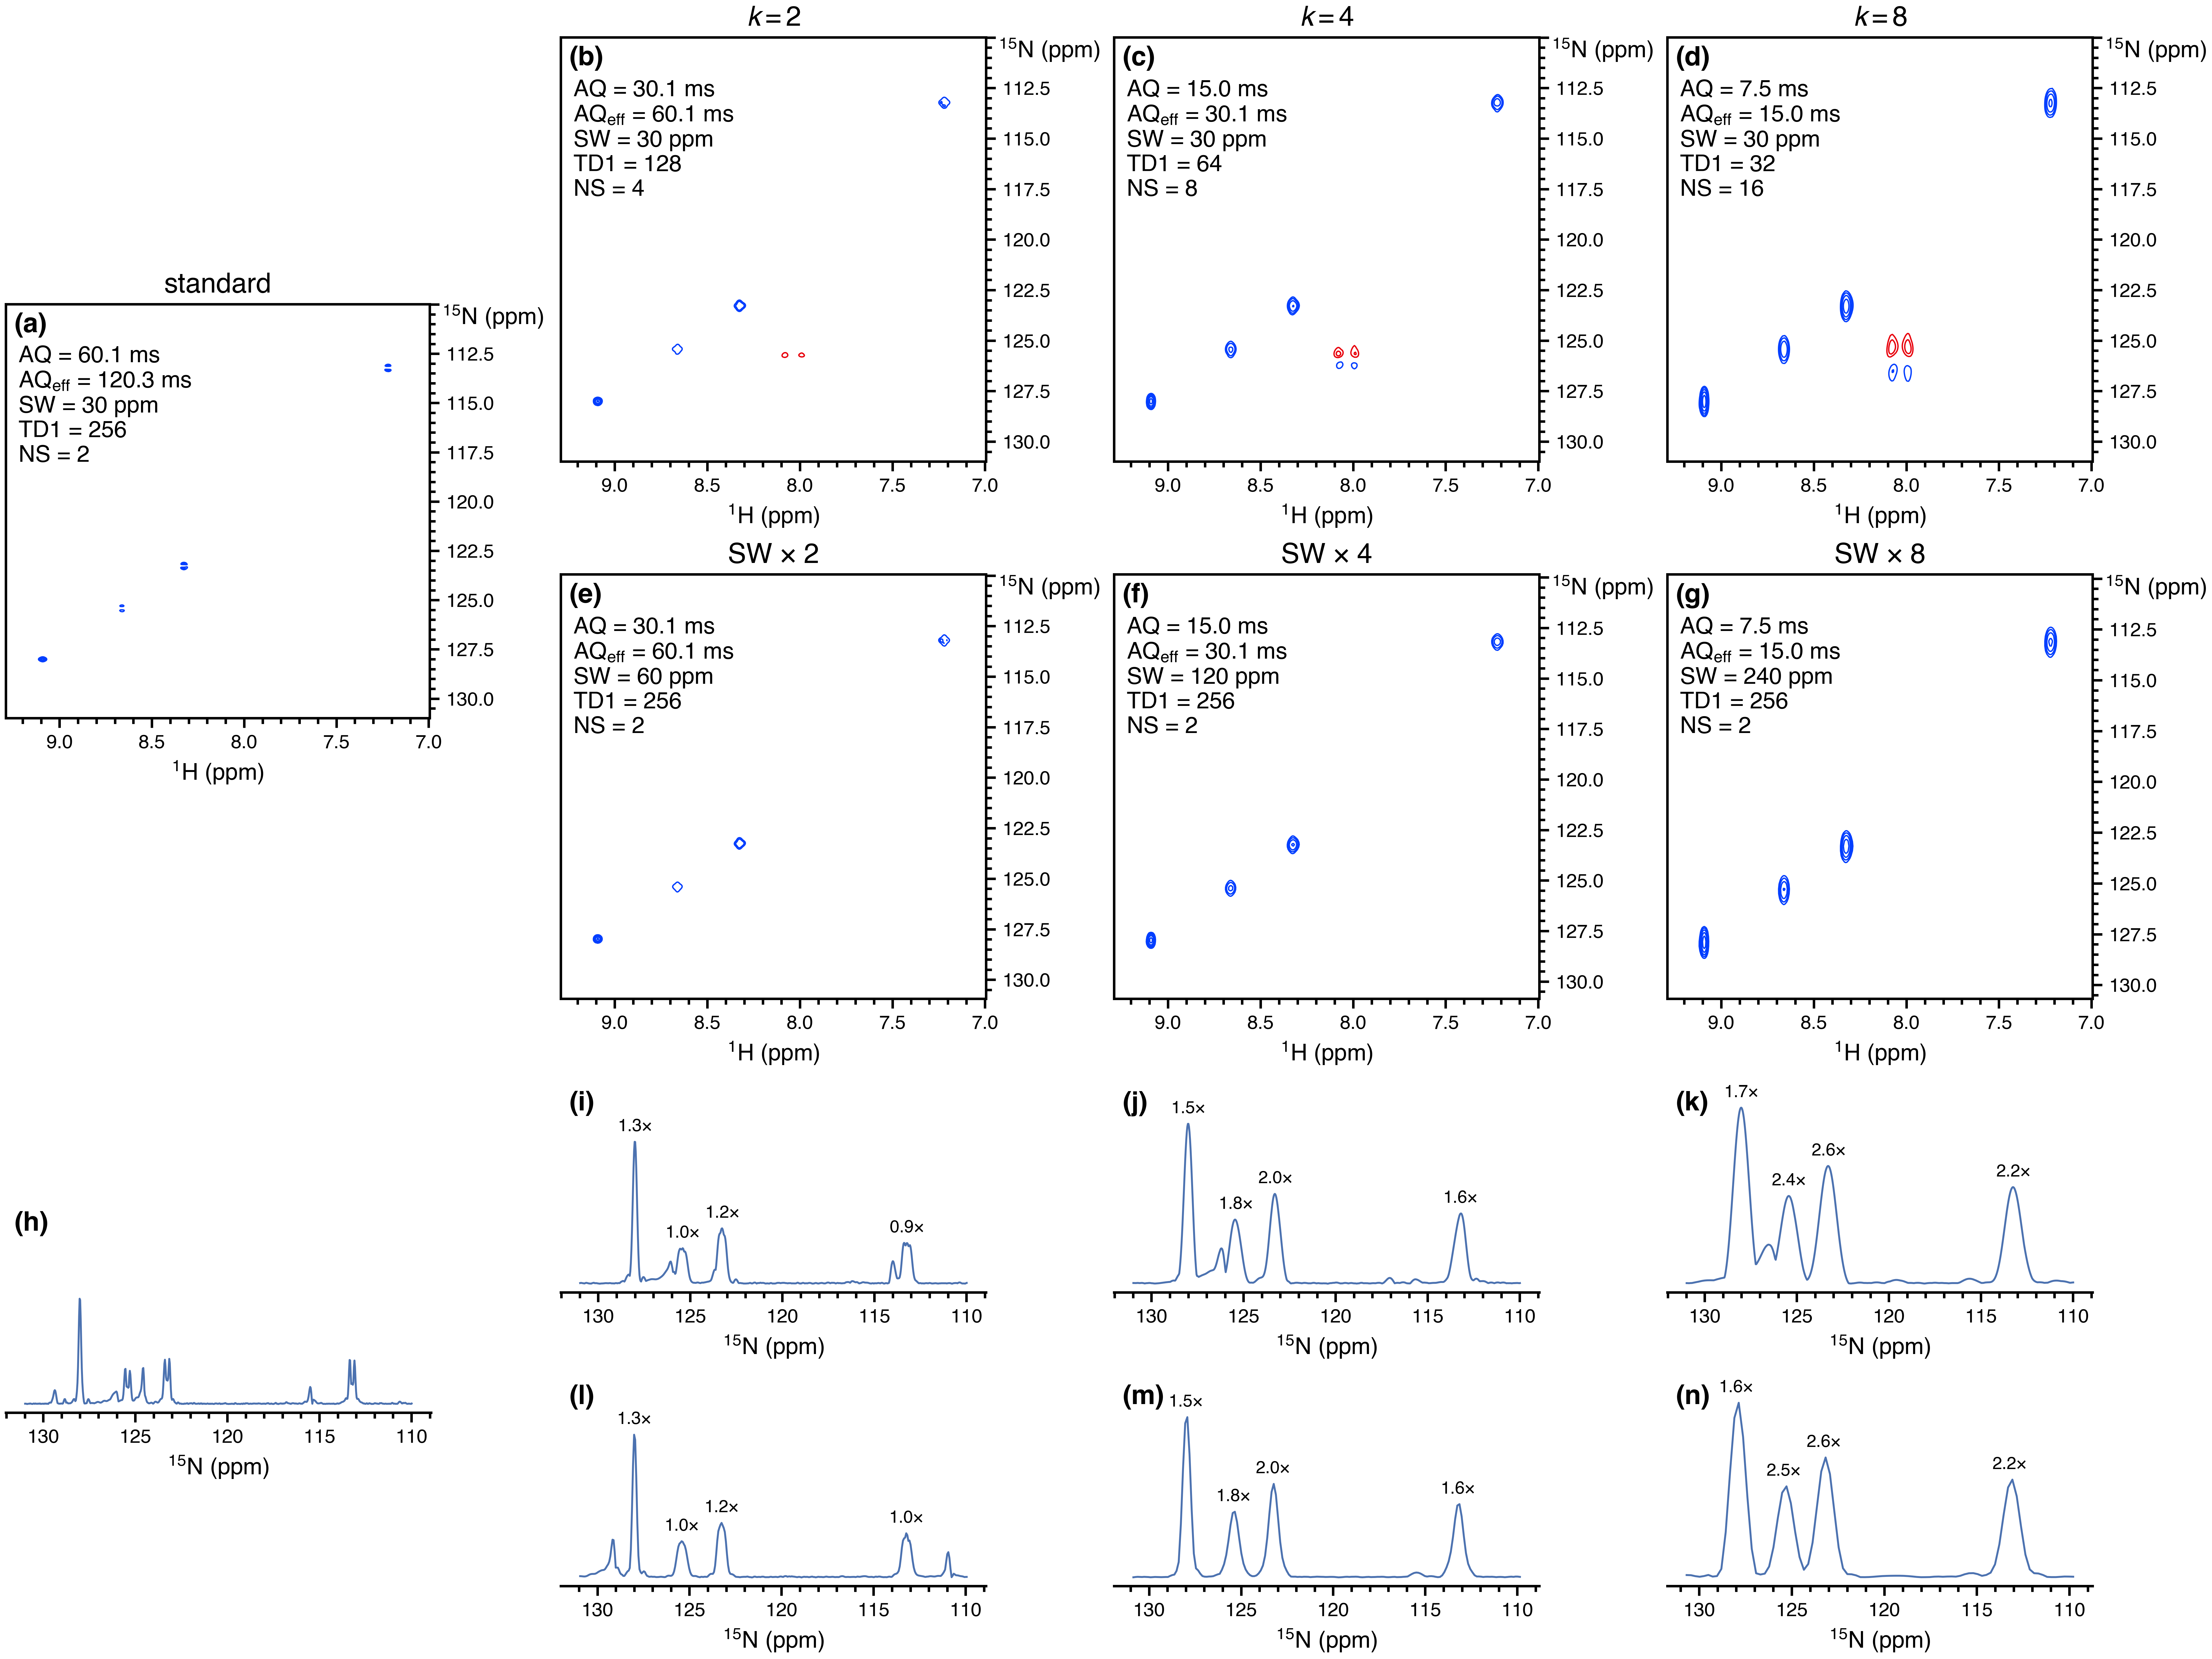
\includegraphics[width=0.75\textwidth]{./figures/hmqc_kscale.png}
    \caption{
        \textbf{(HMQC without linear prediction.)}
        \nitrogen{} HMQC spectra (from NOAH-3 MSpCc supersequences) obtained with various values of the scaling factor $k$.
        The peak at $\Omega_{\ce{H}} = \SI{8.03}{\ppm}$ is a folded peak from the ornithine \textdelta-\ce{NH2}.
        \textbf{(a)} $k = 1$, with 256 $t_1$ increments and 2 scans per increment.
        \textbf{(b)} $k = 2$, i.e.\ effectively 128 $t_1$ increments and 4 scans per increment.
        \textbf{(c)} $k = 4$.
        \textbf{(d)} $k = 8$.
        \textbf{(e)--(h)} Projections of 2D spectra in (a)--(d) onto the $f_1$ axis.
        Numbers indicate peak intensities relative to the $k = 1$ HMQC spectrum.
        \grami{}
    }
    \label{fig:hmqc_kscale}
\end{figure}

\begin{figure}
    \centering
    % figures/spv2_kscale.py
    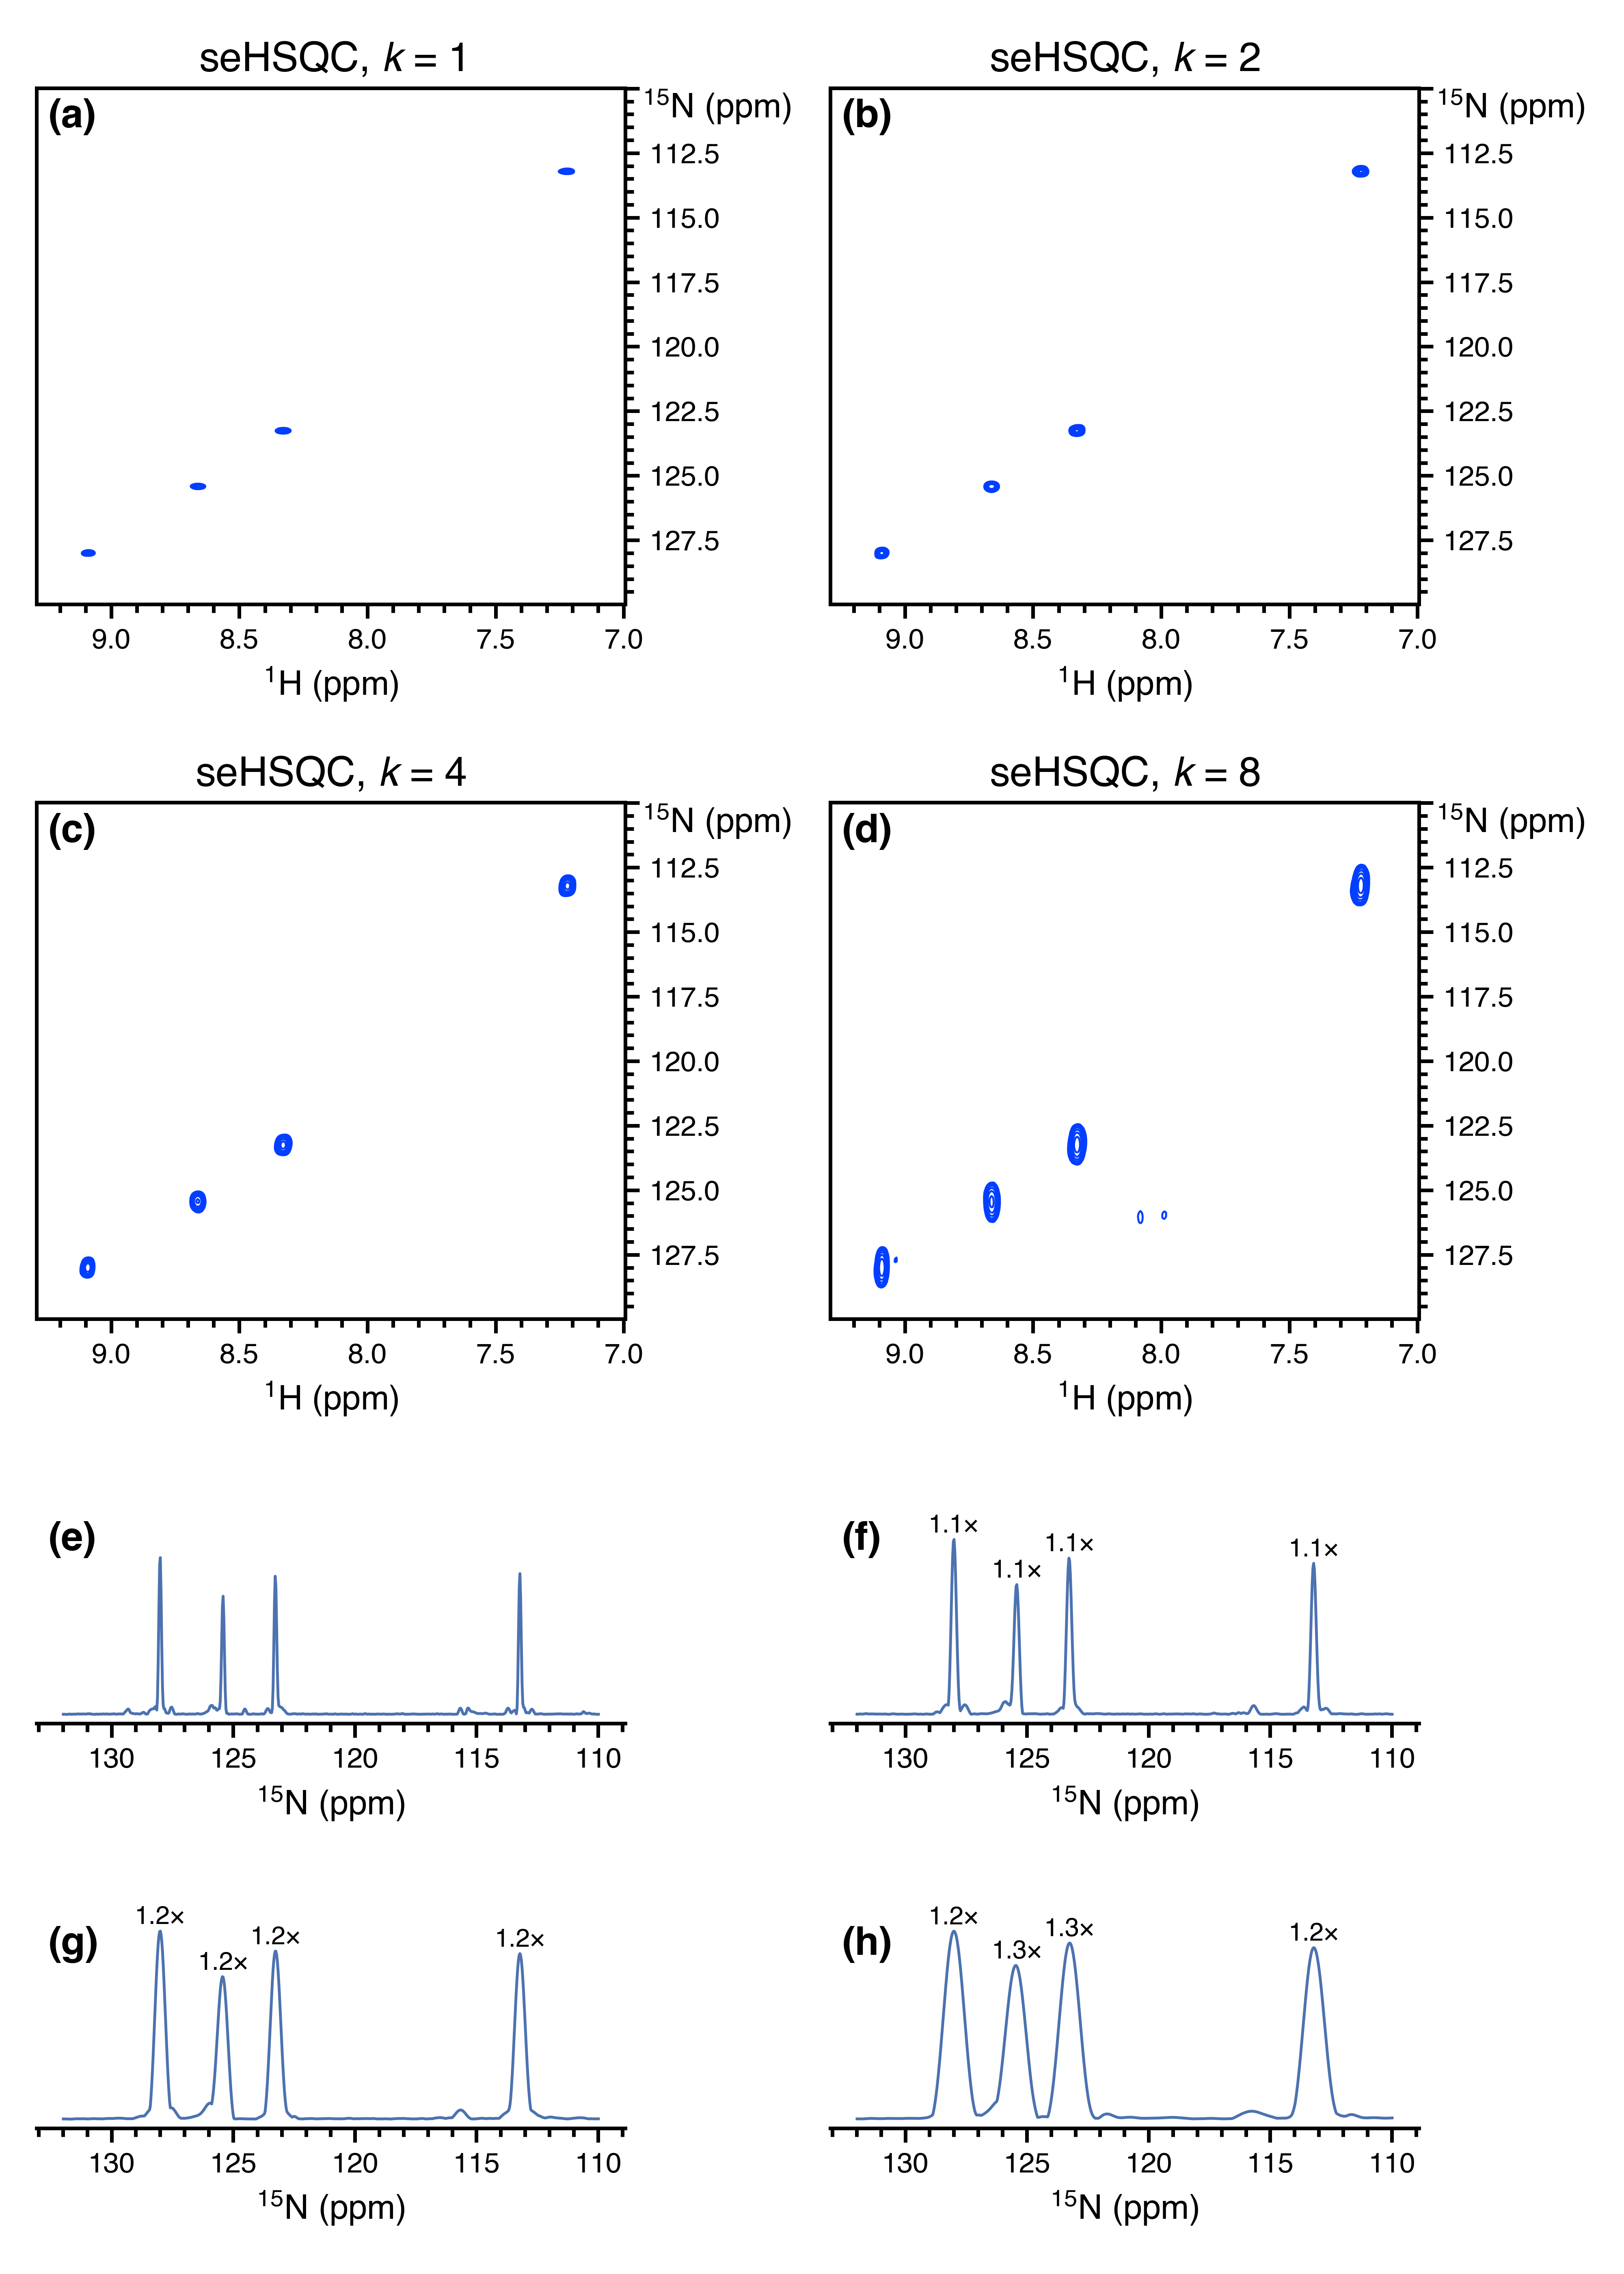
\includegraphics[width=0.75\textwidth]{./figures/spv2_kscale.png}
    \caption{
        \textbf{(seHSQC without linear prediction.)}
        \nitrogen{} seHSQC spectra (from NOAH-3 SpnSpCc supersequences) obtained with various values of the scaling factor $k$.
        The peak at $\Omega_{\ce{H}} = \SI{8.03}{\ppm}$ is a folded peak from the ornithine \textdelta-\ce{NH2}.
        \textbf{(a)} $k = 1$, with 256 $t_1$ increments and 2 scans per increment.
        \textbf{(b)} $k = 2$, i.e.\ effectively 128 $t_1$ increments and 4 scans per increment.
        \textbf{(c)} $k = 4$.
        \textbf{(d)} $k = 8$.
        \textbf{(e)--(h)} Projections of 2D spectra in (a)--(d) onto the $f_1$ axis.
        Numbers indicate peak intensities relative to the $k = 1$ seHSQC spectrum.
        \grami{}
    }
    \label{fig:spv2_kscale}
\end{figure}

\begin{figure}
    \centering
    % figures/hmqc_kscale_lp.py
    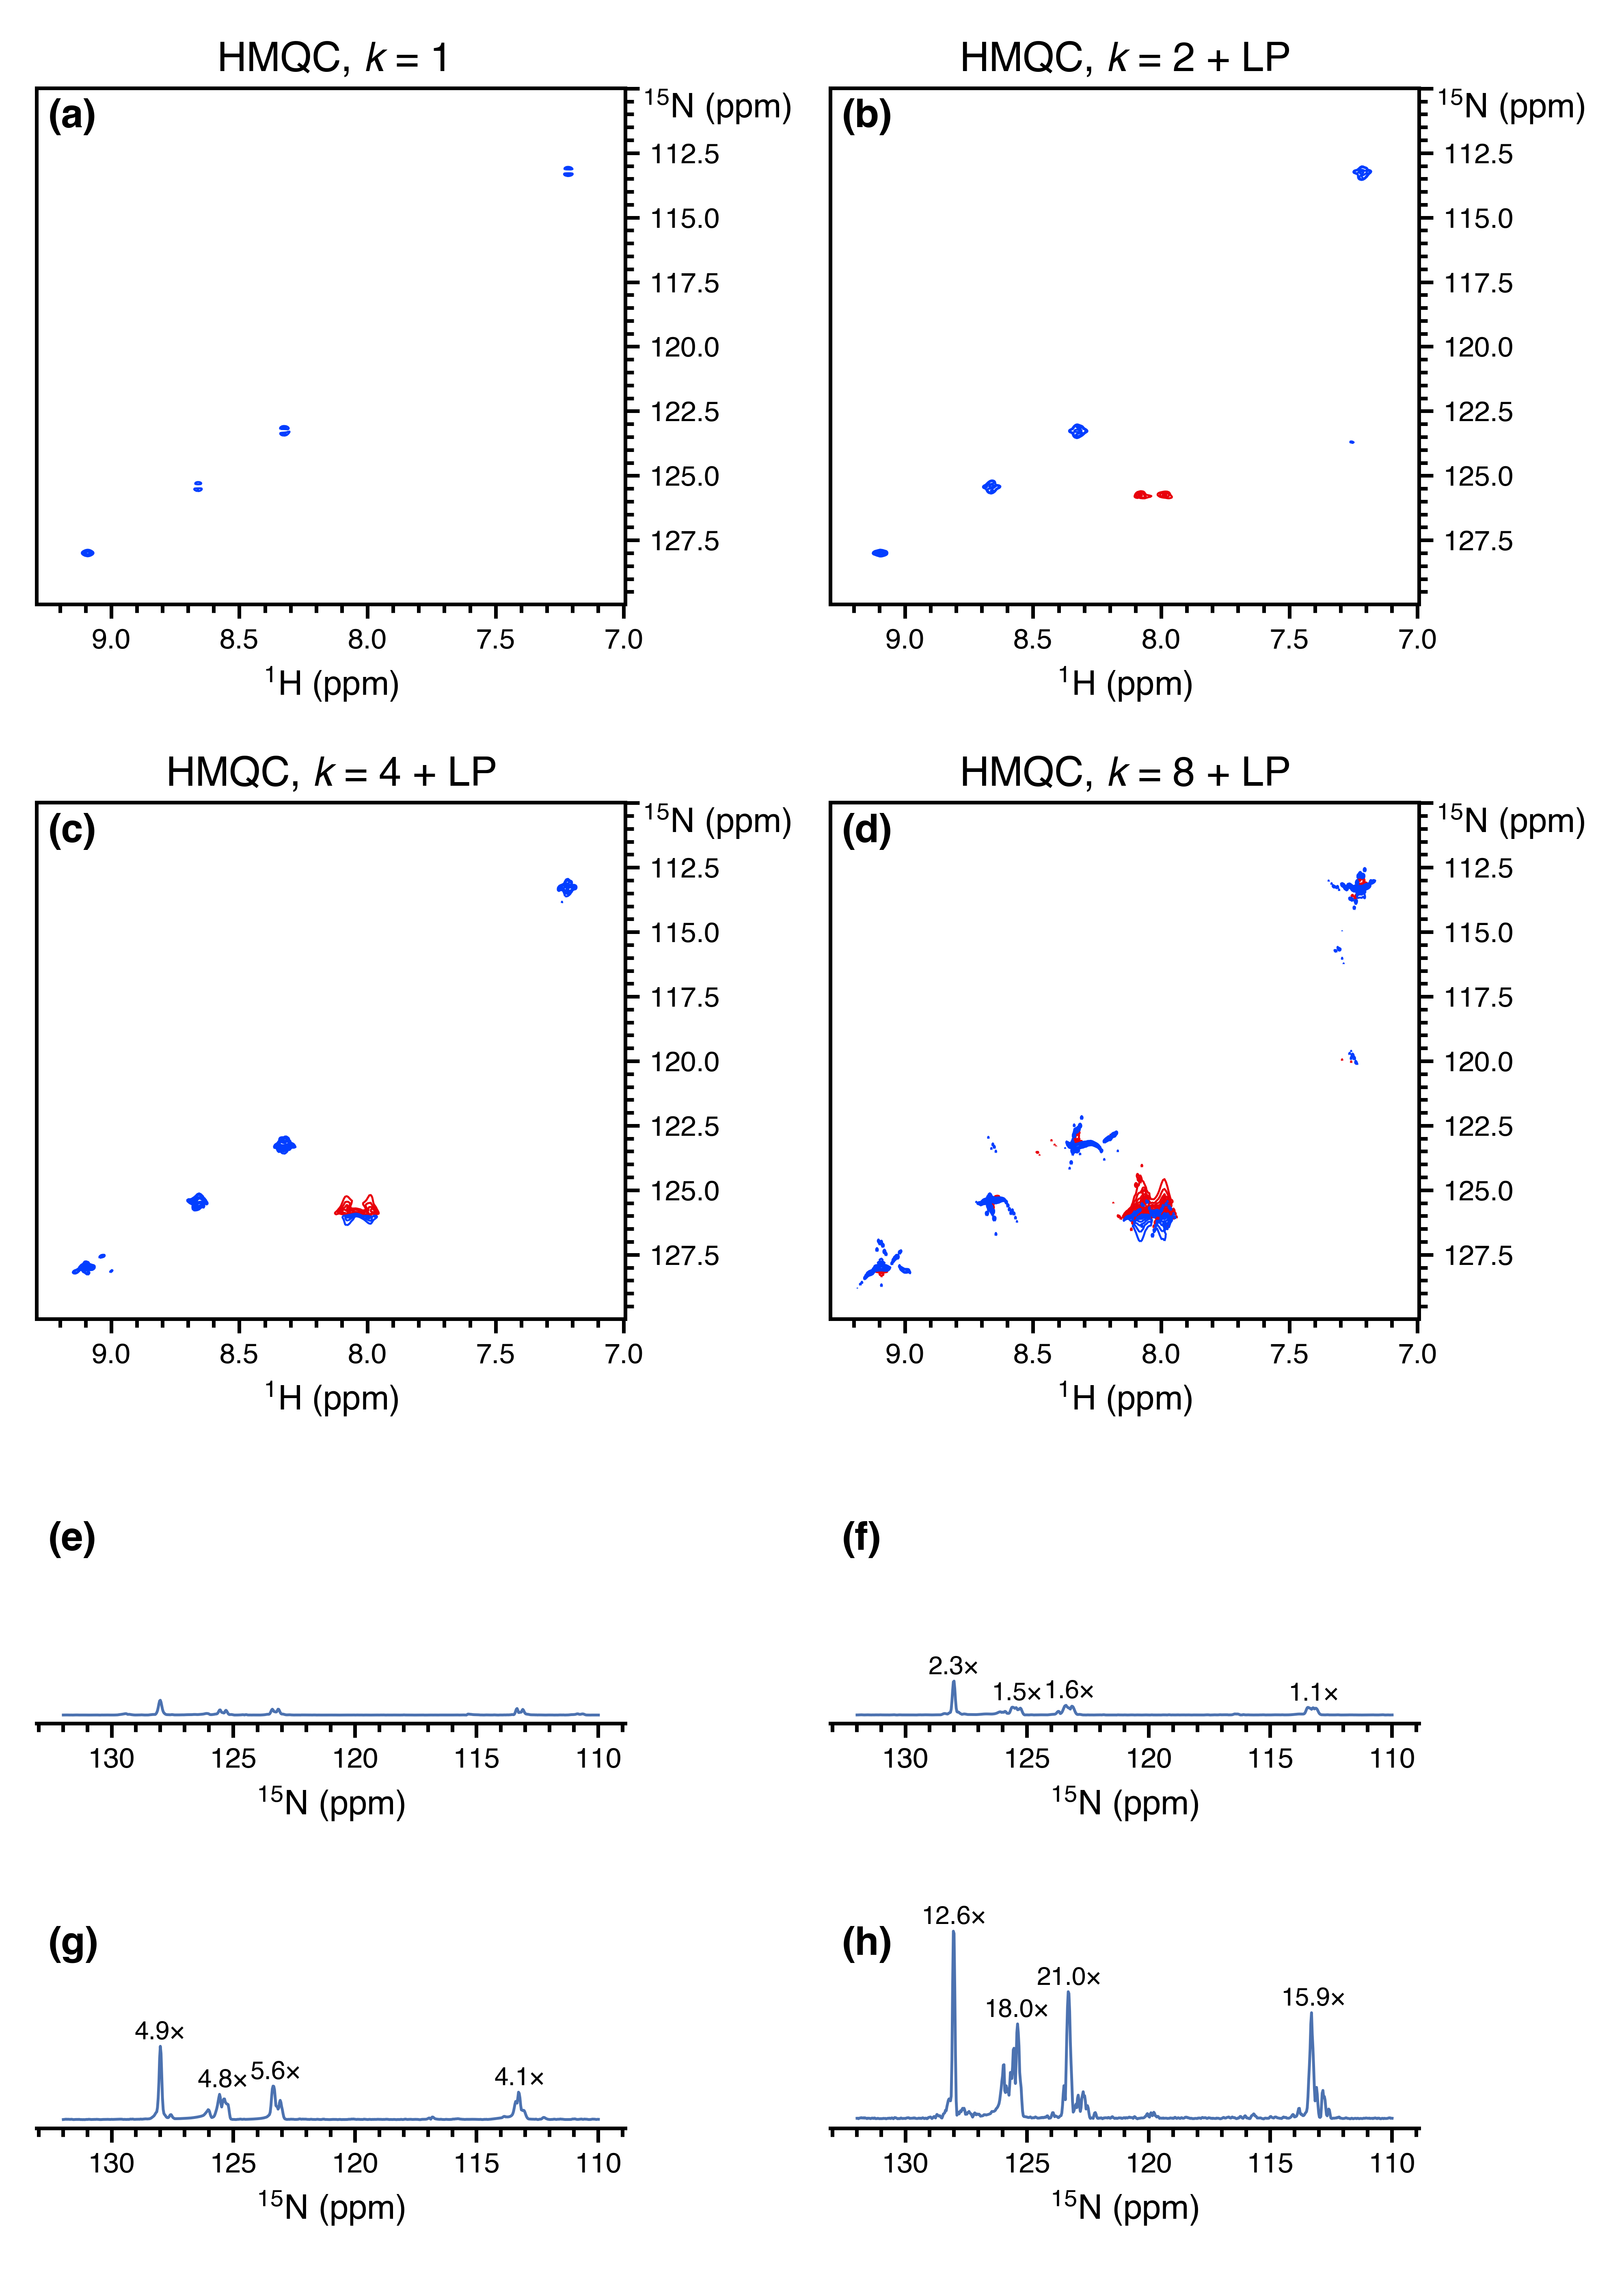
\includegraphics[width=0.75\textwidth]{./figures/hmqc_kscale_lp.png}
    \caption{
        \textbf{(HMQC with linear prediction.)}
        \nitrogen{} HMQC spectra (from NOAH-3 MSpCc supersequences) obtained with various values of the scaling factor $k$, after linear prediction up to 512 complex points in $f_1$.
        The peak at $\Omega_{\ce{H}} = \SI{8.03}{\ppm}$ is a folded peak from the ornithine \textdelta-\ce{NH2}.
        \textbf{(a)} $k = 1$. Note that this spectrum is the same as in \figref{hmqc_kscale}a.
        \textbf{(b)} $k = 2$.
        \textbf{(c)} $k = 4$.
        \textbf{(d)} $k = 8$.
        \textbf{(e)--(h)} Projections of 2D spectra in (a)--(d) onto the $f_1$ axis.
        Numbers indicate peak intensities relative to the $k = 1$ HMQC spectrum.
        \grami{}
    }
    \label{fig:hmqc_kscale_lp}
\end{figure}

\begin{figure}
    \centering
    % figures/spv2_kscale_lp.py
    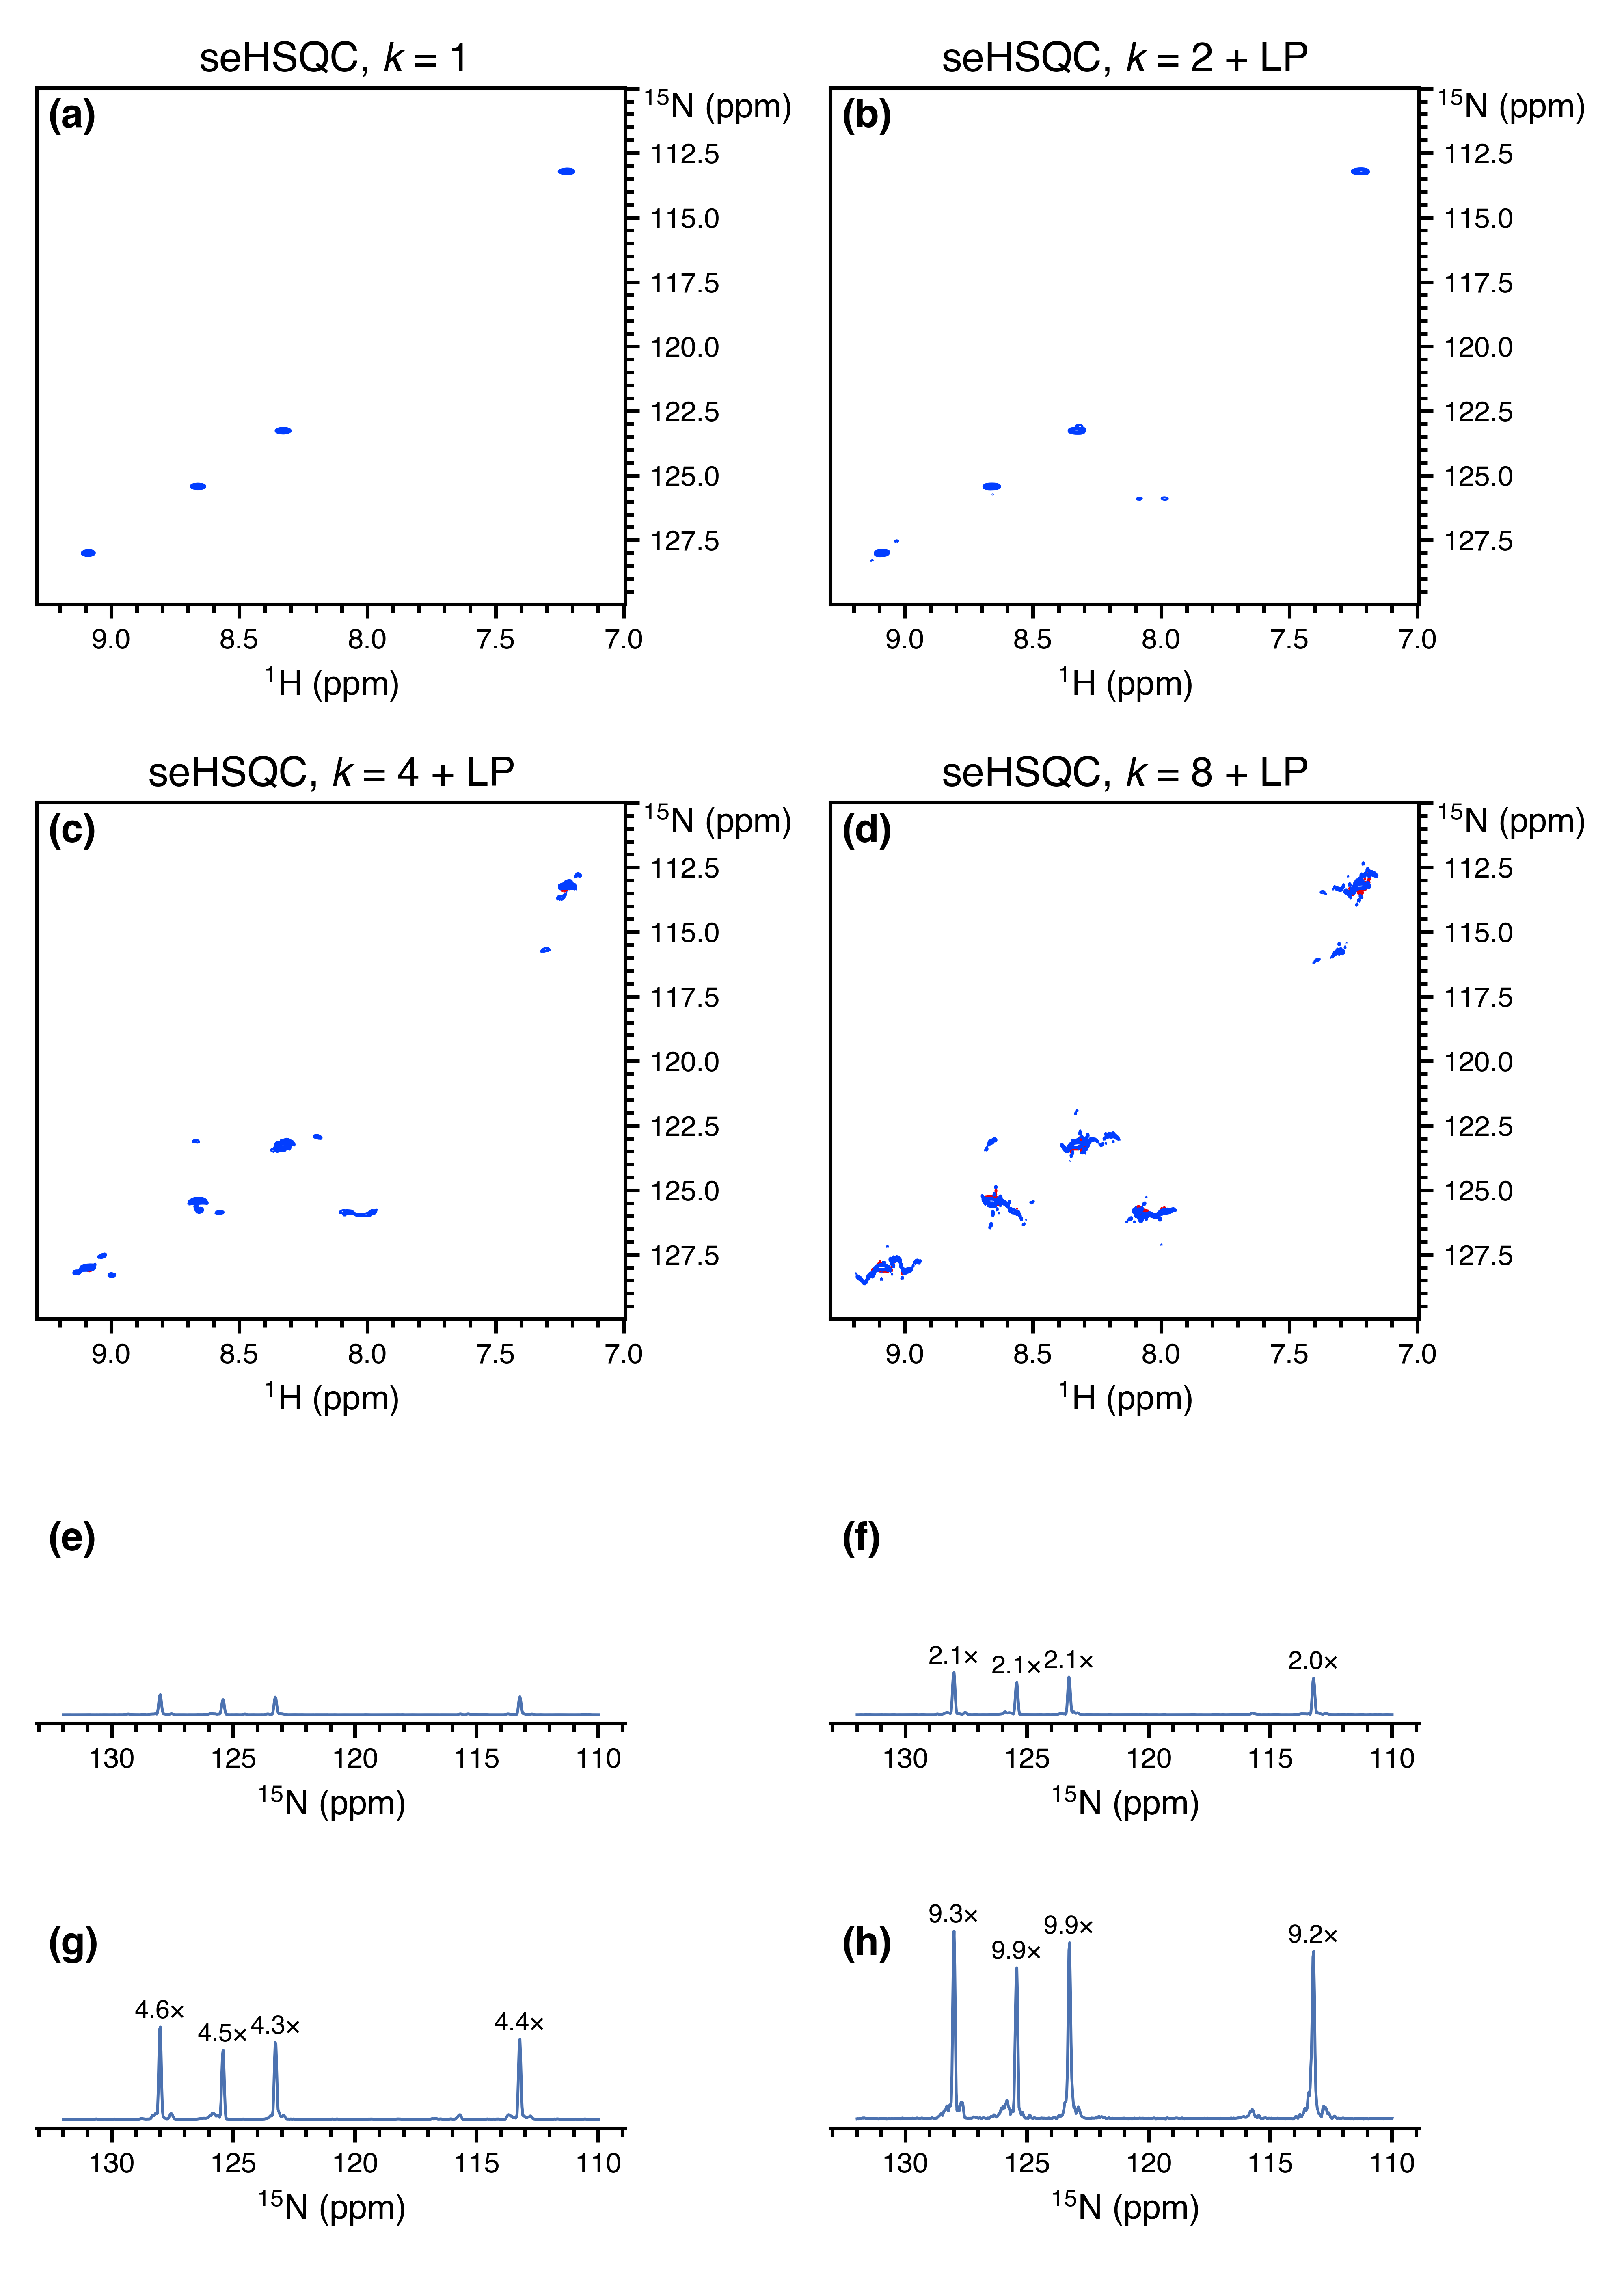
\includegraphics[width=0.75\textwidth]{./figures/spv2_kscale_lp.png}
    \caption{
        \textbf{(seHSQC with linear prediction.)}
        \nitrogen{} seHSQC spectra (from NOAH-3 SpnSpCc supersequences) obtained with various values of the scaling factor $k$, after linear prediction up to 512 complex points in $f_1$.
        The peak at $\Omega_{\ce{H}} = \SI{8.03}{\ppm}$ is a folded peak from the ornithine \textdelta-\ce{NH2}.
        \textbf{(a)} $k = 1$. Note that this spectrum is the same as in \figref{hmqc_kscale}a.
        \textbf{(b)} $k = 2$.
        \textbf{(c)} $k = 4$.
        \textbf{(d)} $k = 8$.
        \textbf{(e)--(h)} Projections of 2D spectra in (a)--(d) onto the $f_1$ axis.
        Numbers indicate peak intensities relative to the $k = 1$ seHSQC spectrum.
        \grami{}
    }
    \label{fig:spv2_kscale_lp}
\end{figure}

\section{HSQC-TOCSY/HSQC sensitivity comparisons}

The signal intensities for the NOAH-3 StSCc (HSQC-TOCSY + HSQC + CLIP-COSY) supersequences can be more conveniently measured by omitting the DIPSI-2 isotropic mixing in the HSQC-TOCSY supersequence, leading to a NOAH-3 SSCc (HSQC + HSQC + CLIP-COSY) supersequence.
This allows us to compare the different versions of double-HSQC sequences, as the two HSQC modules can be implemented either using the MFA approach, or the new ASAP/NOAH approach based on Ernst angle excitation in the first module.
In the latter implementation, the parameter $f$ can be varied between 0.4 and 1; it represents the proportion of \carbon{}--\proton{} magnetisation used in the first HSQC, as described in the main text.
Furthermore, to boost the sensitivity of the second HSQC module in the NOAH supersequences, the new seHSQC module can be used in place of it.

\begin{figure}
    \centering
    % figures/ssc_comparisons.py
    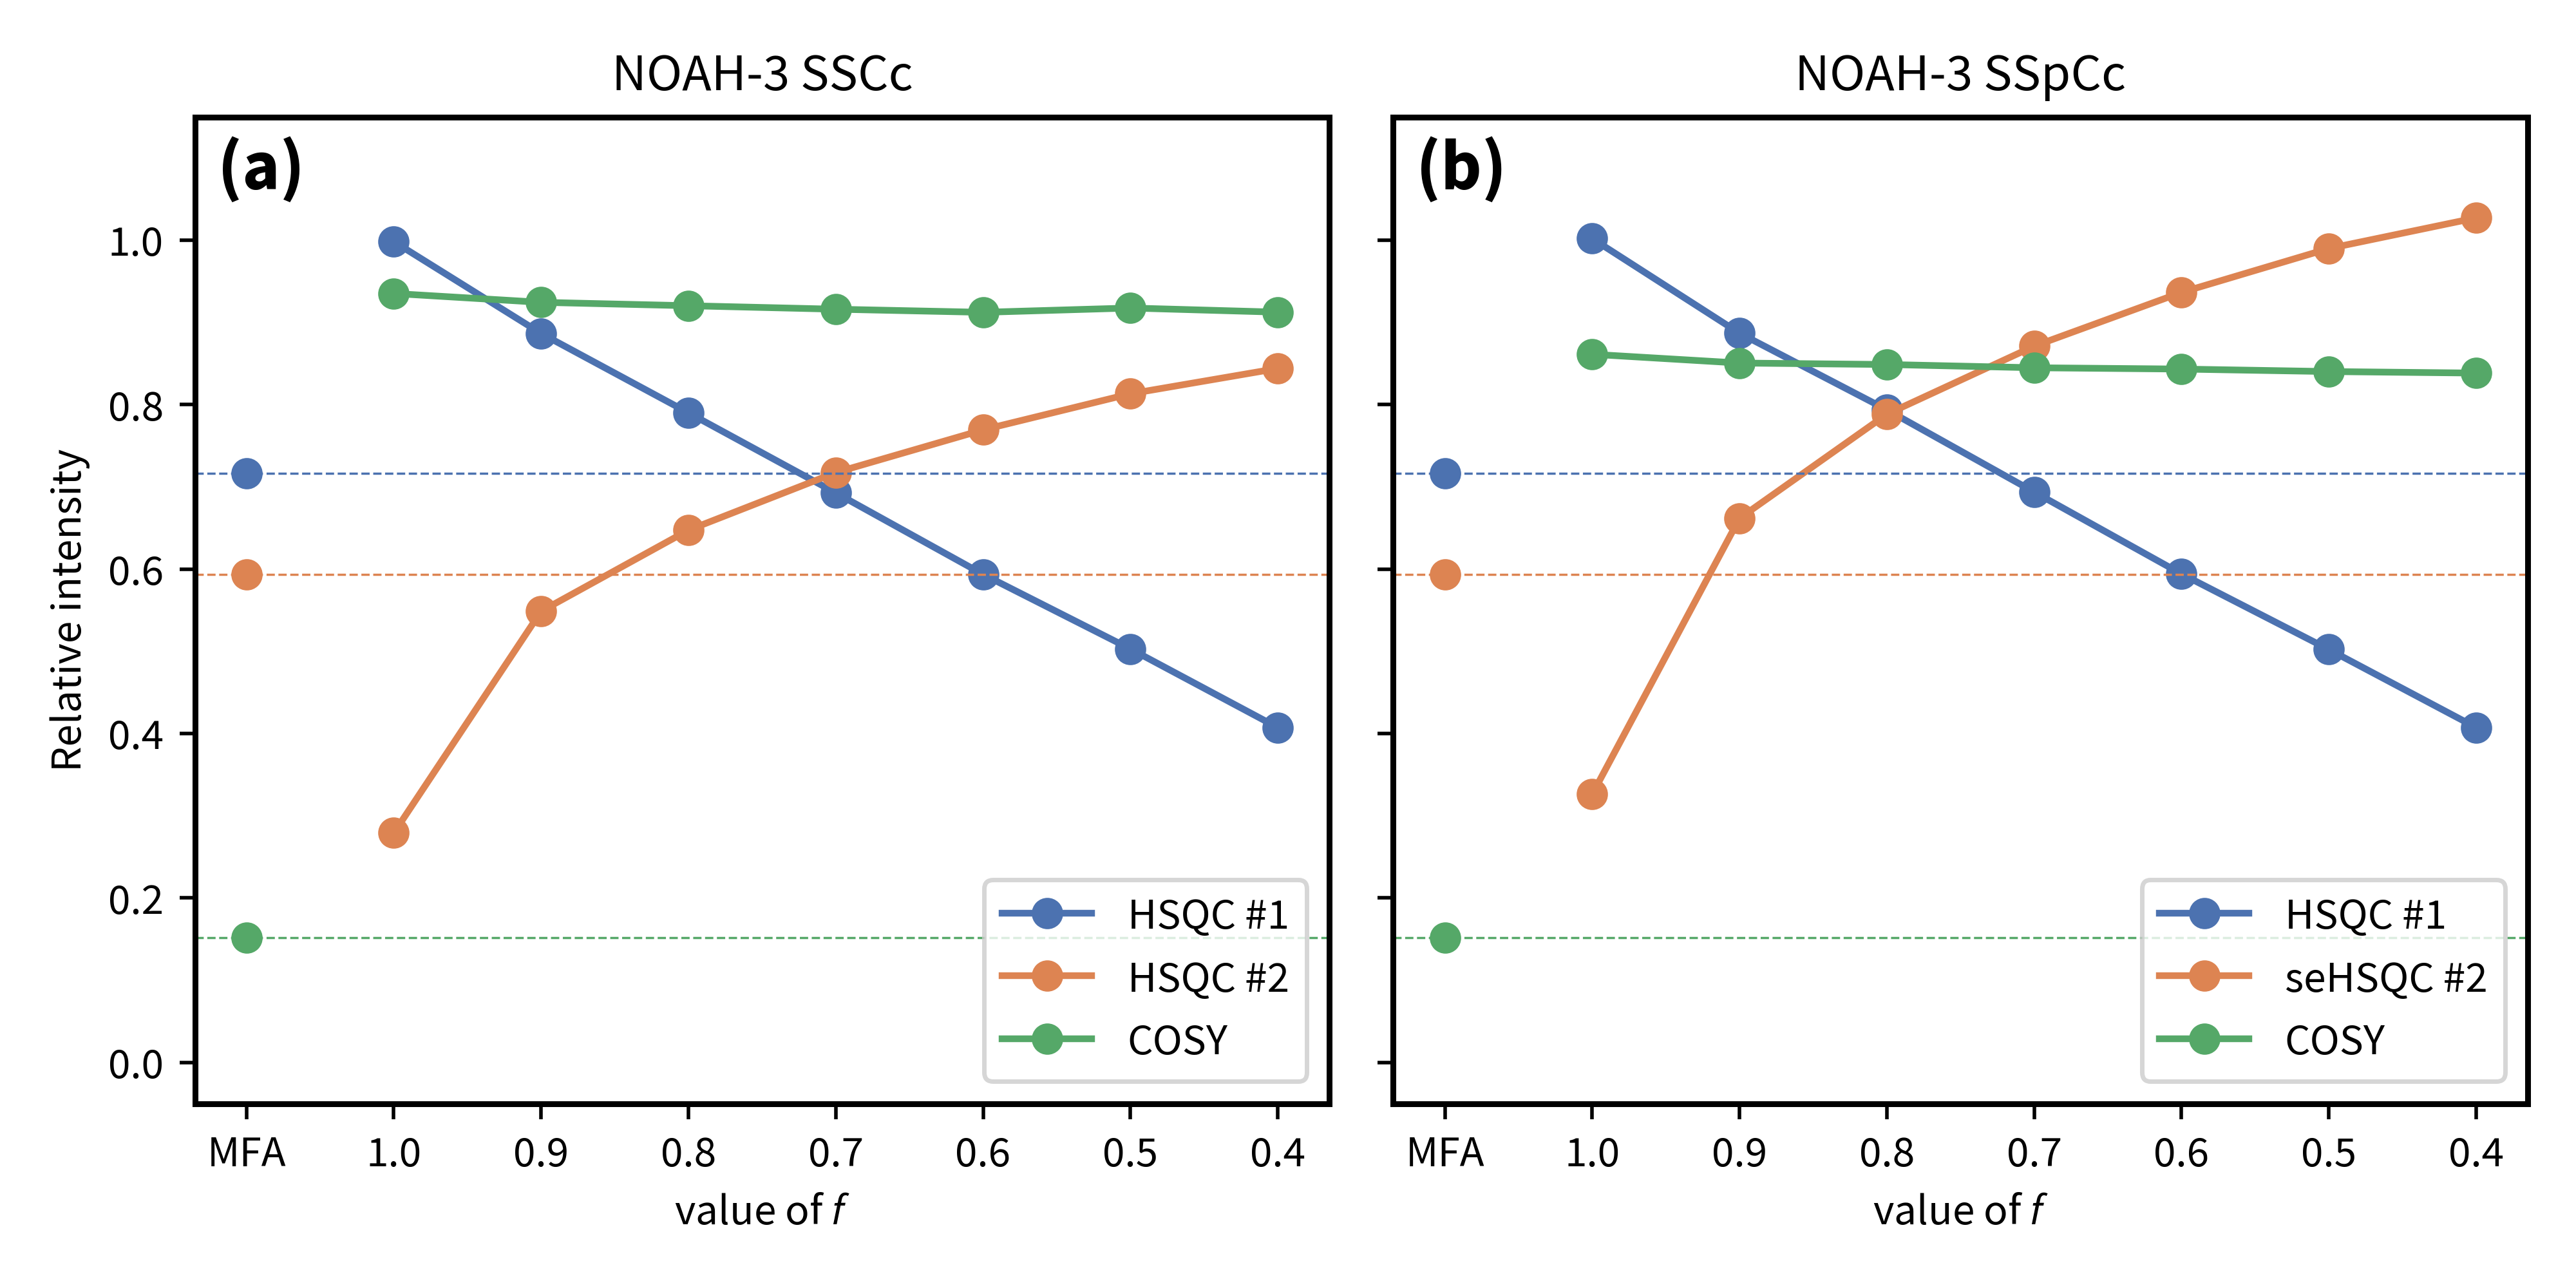
\includegraphics[width=0.8\textwidth]{./figures/ssc_comparisons.png}
    \caption{
        Sensitivities of HSQC and CLIP-COSY modules when used as part of a SSCc-type supersequence, with both the NOAH and MFA implementations of the two HSQC modules.
        Intensities are calculated relative to the HSQC and CLIP-COSY modules in a standard NOAH-2 SCc supersequence (averaged over all peaks).
        The MFA SSCc sensitivies are on the left of each plot; horizontal dashed lines at these levels are drawn to guide the eye.
        \textbf{(a)} Sensitivity of NOAH-3 SSCc modules as a function of $f$.
        \textbf{(b)} Sensitivity of NOAH-3 SSpCc modules (the second HSQC module is replaced with seHSQC) as a function of $f$.
        \andro{}
    }
    \label{fig:ssc_comparisons}
\end{figure}

\figref{ssc_comparisons} can be understood in the following way:

\begin{itemize}
    \item The MFA HSQC sensitivities (on the left of both plots) are approximately half that of a standard CRK seHSQC, with the second HSQC having slightly lower sensitivity.
        This is discussed in ref.\ \citenum{Nolis2019CPC} of the main text.
    \item The sensitivity of the first NOAH HSQC (blue) is generally equal to $f$, supporting the interpretation of $f$ as the fraction of \carbon{}--\proton{} magnetisation excited in the first HSQC.
    \item The sensitivity of the second NOAH HSQC (orange) arises from whatever is \textit{not} used by the first HSQC, plus any magnetisation that relaxes during the FID of the first HSQC.
        As $f$ is decreased, the former contribution increases and the latter tapers off.
        This is true for the seHSQC as well (in \figref{ssc_comparisons}b), except that there is a uniform boost in sensitivity for all values of $f$.
        This sensitivity improvement mainly applies to \ce{CH} groups, as discussed in the main text.
    \item The MFA COSY sensitivity is substantially lower ($\sim 15\%$) because the bulk magnetisation is dephased by the previous modules, whereas in the NOAH approach it is (largely) preserved.
\end{itemize}

It remains to evaluate the impact of adding DIPSI-2 mixing in one of the HSQC modules on the remaining modules in the supersequence.
This depends on whether the HSQC-TOCSY module is placed first (StSC or StSpC) or second (SStC) in the sequence.
Because of the possibility of using the seHSQC module in the other slot, we generally recommend placing the HSQC-TOCSY sequence first.
As can be seen \hl{TODO}

\begin{figure}
    \centering
    % figures/stsc_comparisons.py
    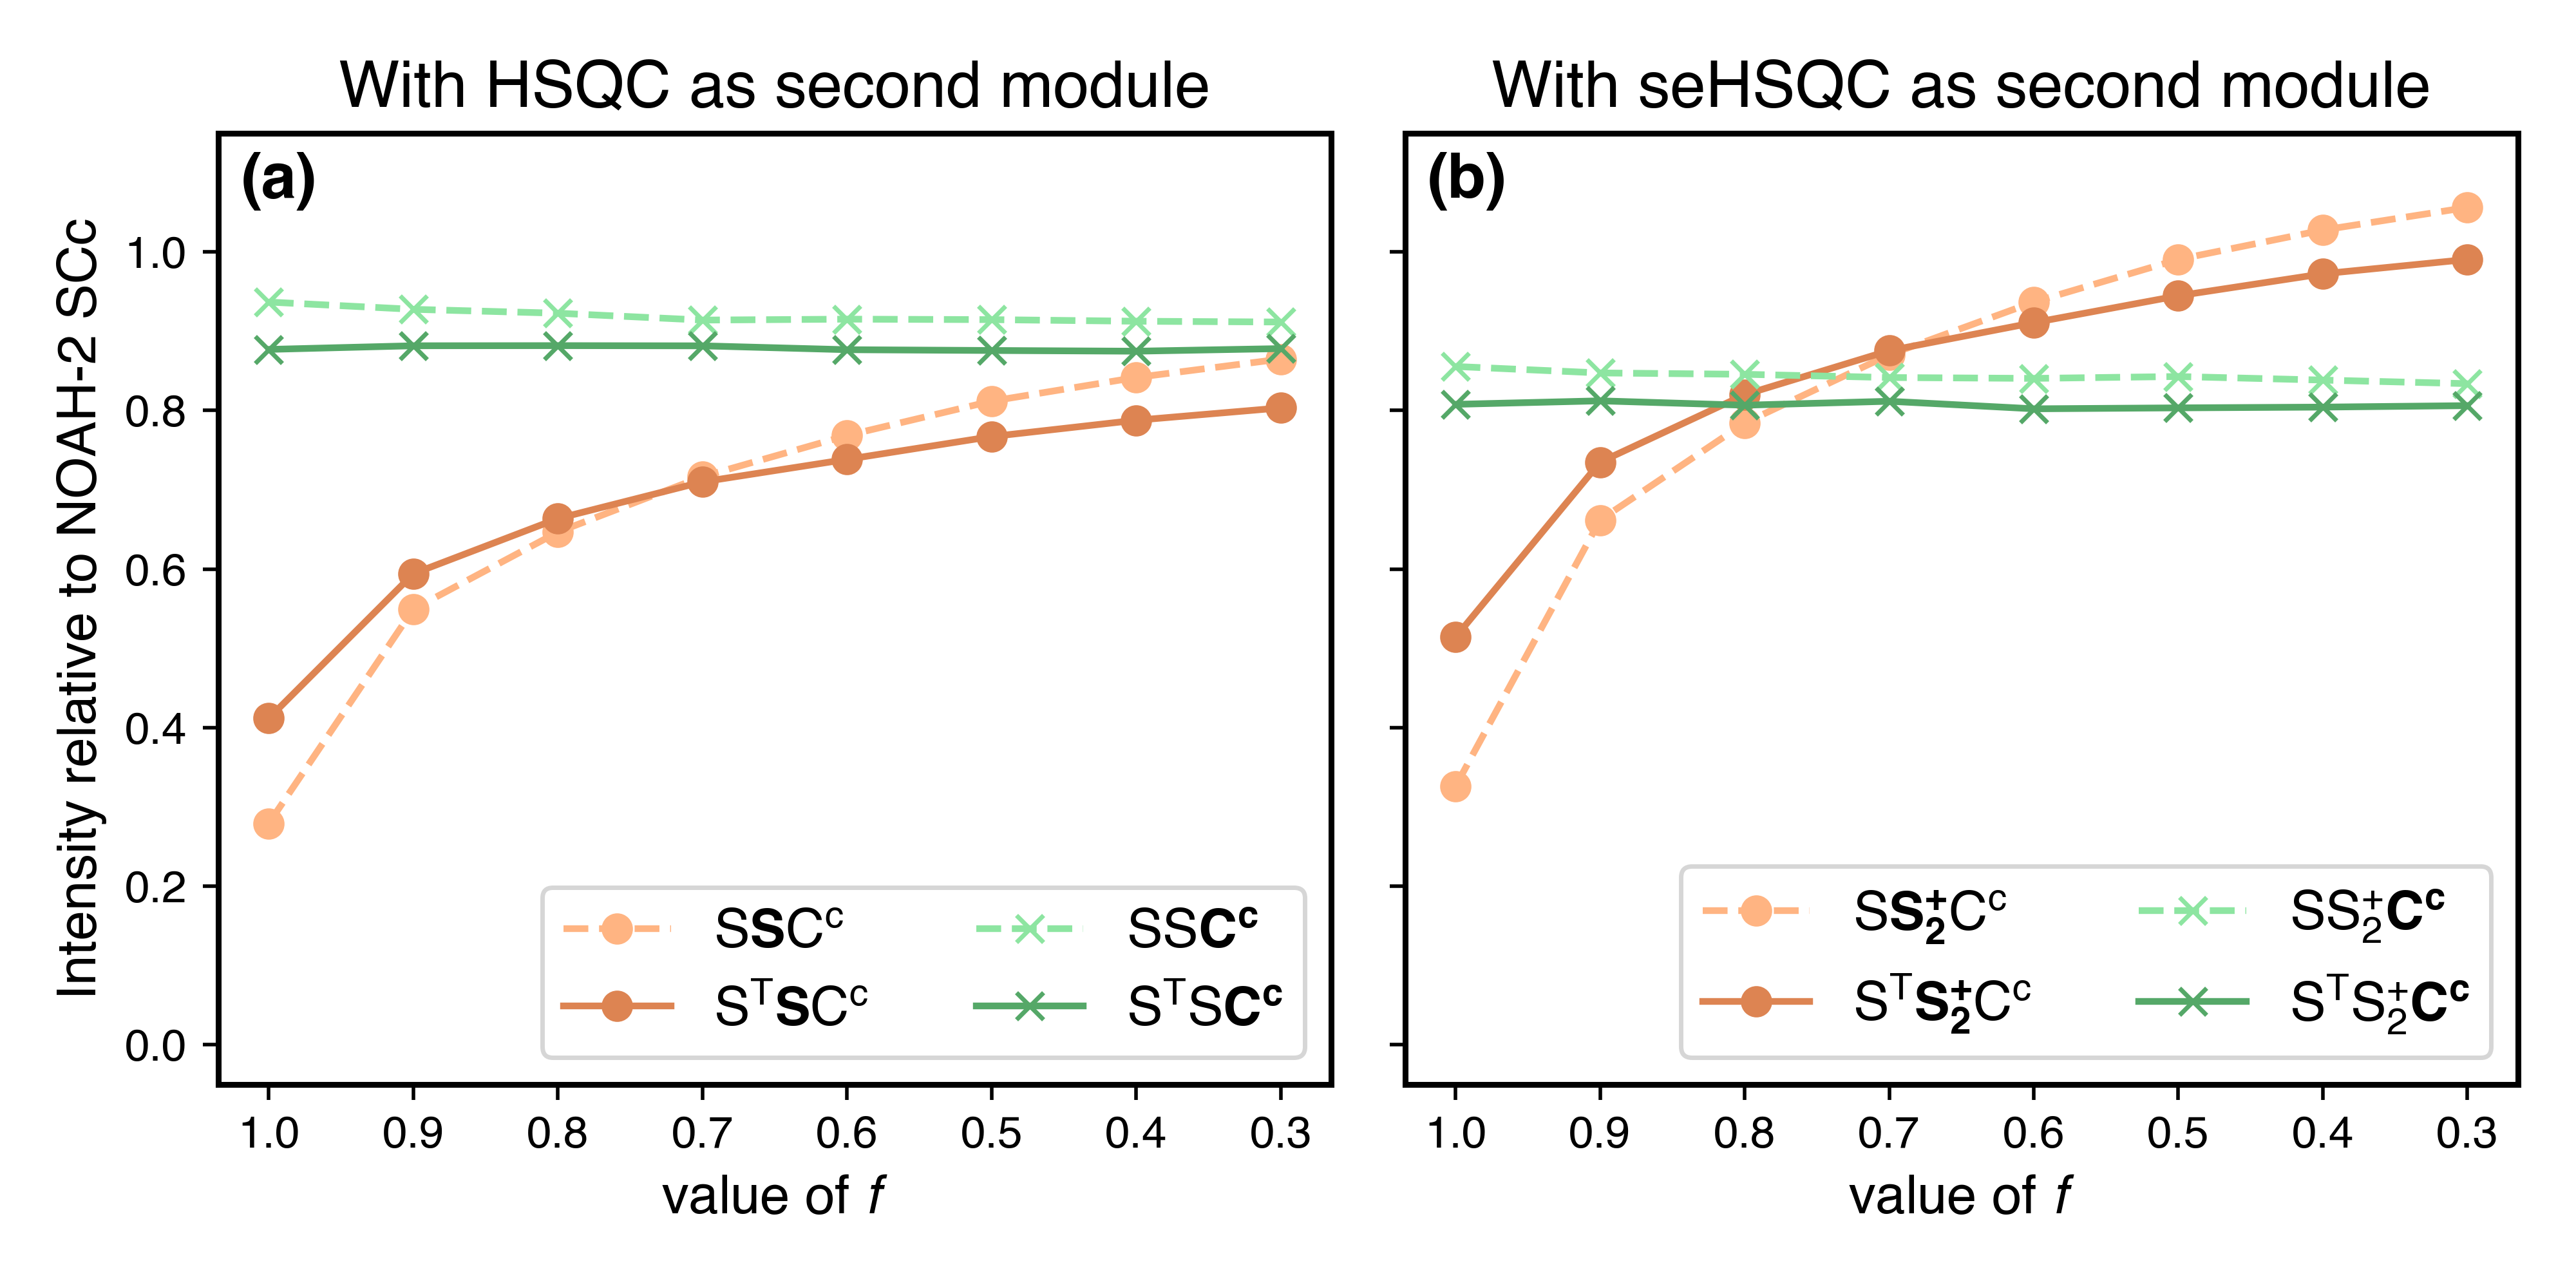
\includegraphics[width=0.8\textwidth]{./figures/stsc_comparisons.png}
    \caption{
        Blah.
        \andro{}
    }
    \label{fig:stsc_comparisons}
\end{figure}

\section{Other example spectra}
\label{section:si_spectra}

\begin{figure}
    \centering
    % figures/stspct.py
    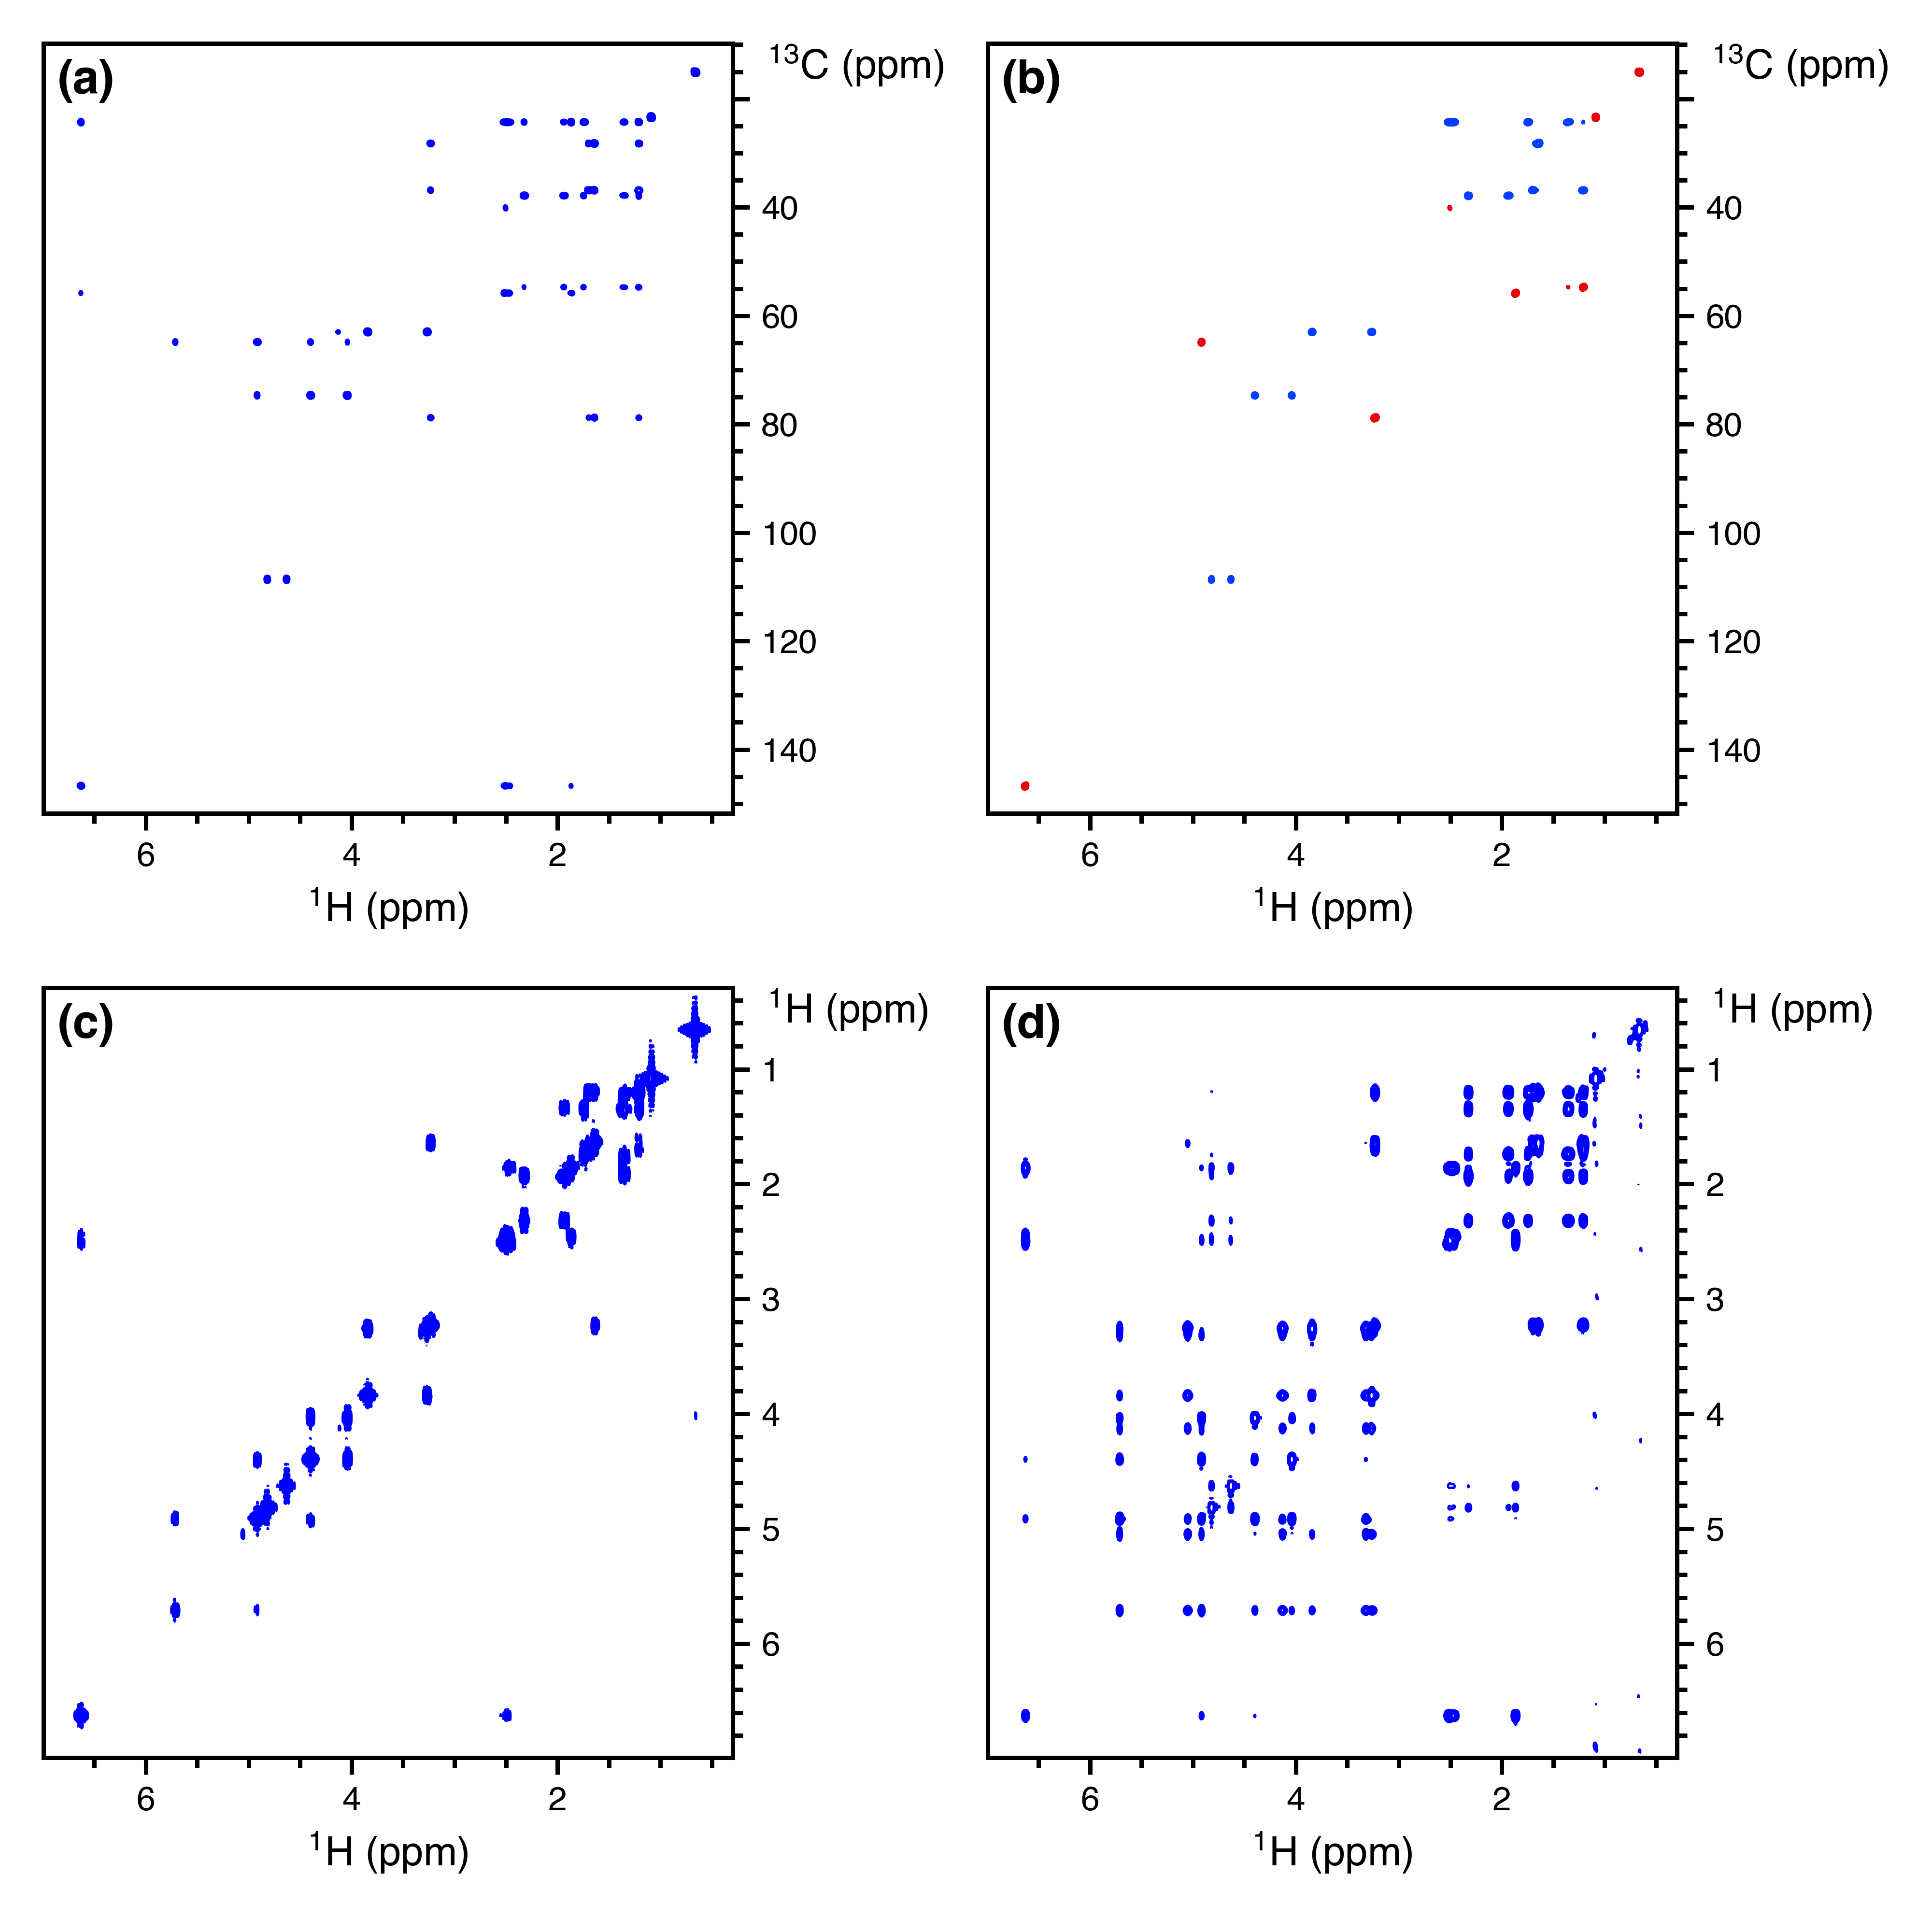
\includegraphics[width=0.8\textwidth]{./figures/stspct.png}
    \caption{
        2D spectra acquired using the NOAH-4 StSpCT supersequence.
        256 $t_1$ increments were used with 2 scans per increment, leading to a total experiment time of 17 minutes and 32 seconds.
        This represents a $3.25\times$ time saving relative to conventional acquisition of each of the four spectra with the same parameters, which would take a total of 57 minutes and 3 seconds.
        \textbf{(a)} HSQC-TOCSY (\SI{30}{ms} mixing time, $f = 0.9$).
        \textbf{(b)} Multiplicity edited seHSQC.
        \textbf{(c)} COSY.
        \textbf{(d)} TOCSY (\SI{60}{ms} mixing time).
        \andro{}
    }
    \label{fig:stspct}
\end{figure}

\begin{figure}
    \centering
    % figures/stspct_nus.py
    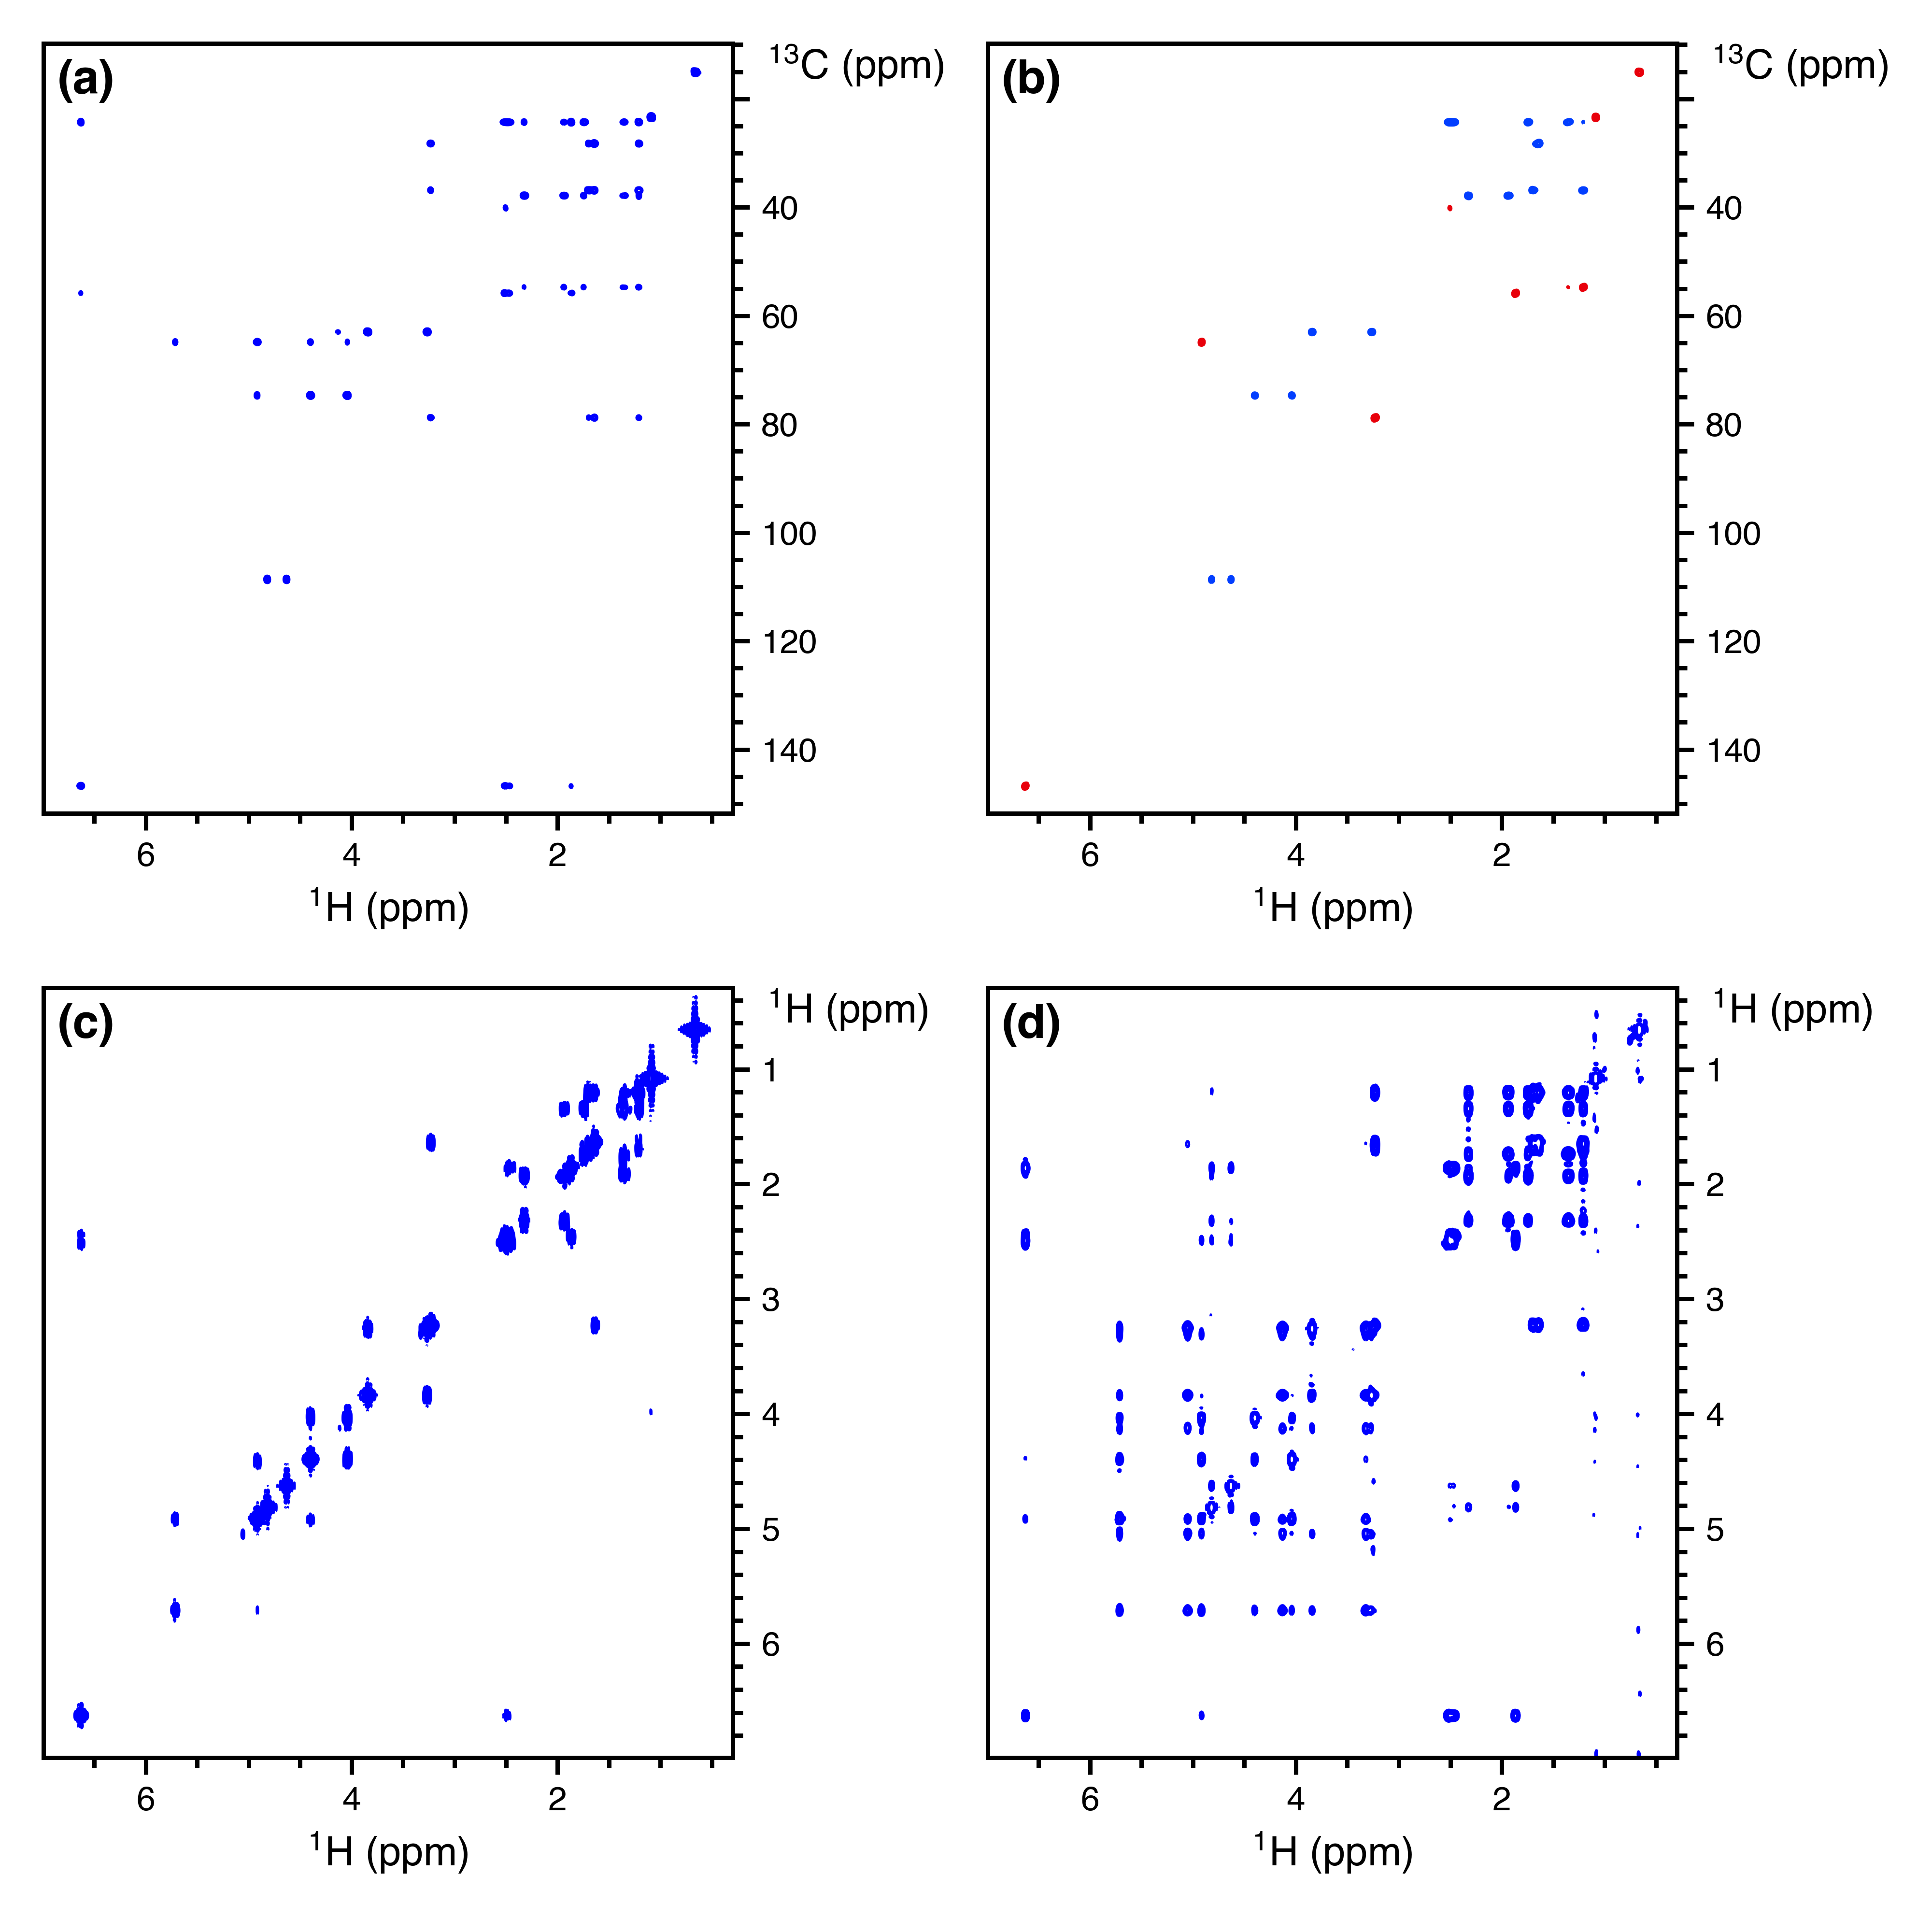
\includegraphics[width=0.8\textwidth]{./figures/stspct_nus.png}
    \caption{
        2D spectra acquired using the NOAH-4 StSpCT supersequence with 50\% non-uniform sampling.
        All other parameters are the same as in \figref{stspct}.
        The experimental time was 9 minutes and 1 second.
        \textbf{(a)} HSQC-TOCSY (\SI{30}{ms} mixing time, $f = 0.9$).
        \textbf{(b)} Multiplicity edited seHSQC.
        \textbf{(c)} COSY.
        \textbf{(d)} TOCSY (\SI{60}{ms} mixing time).
        \andro{}
    }
    \label{fig:stspct_nus}
\end{figure}

\begin{figure}
    \centering
    % figures/bspnspcqf.py
    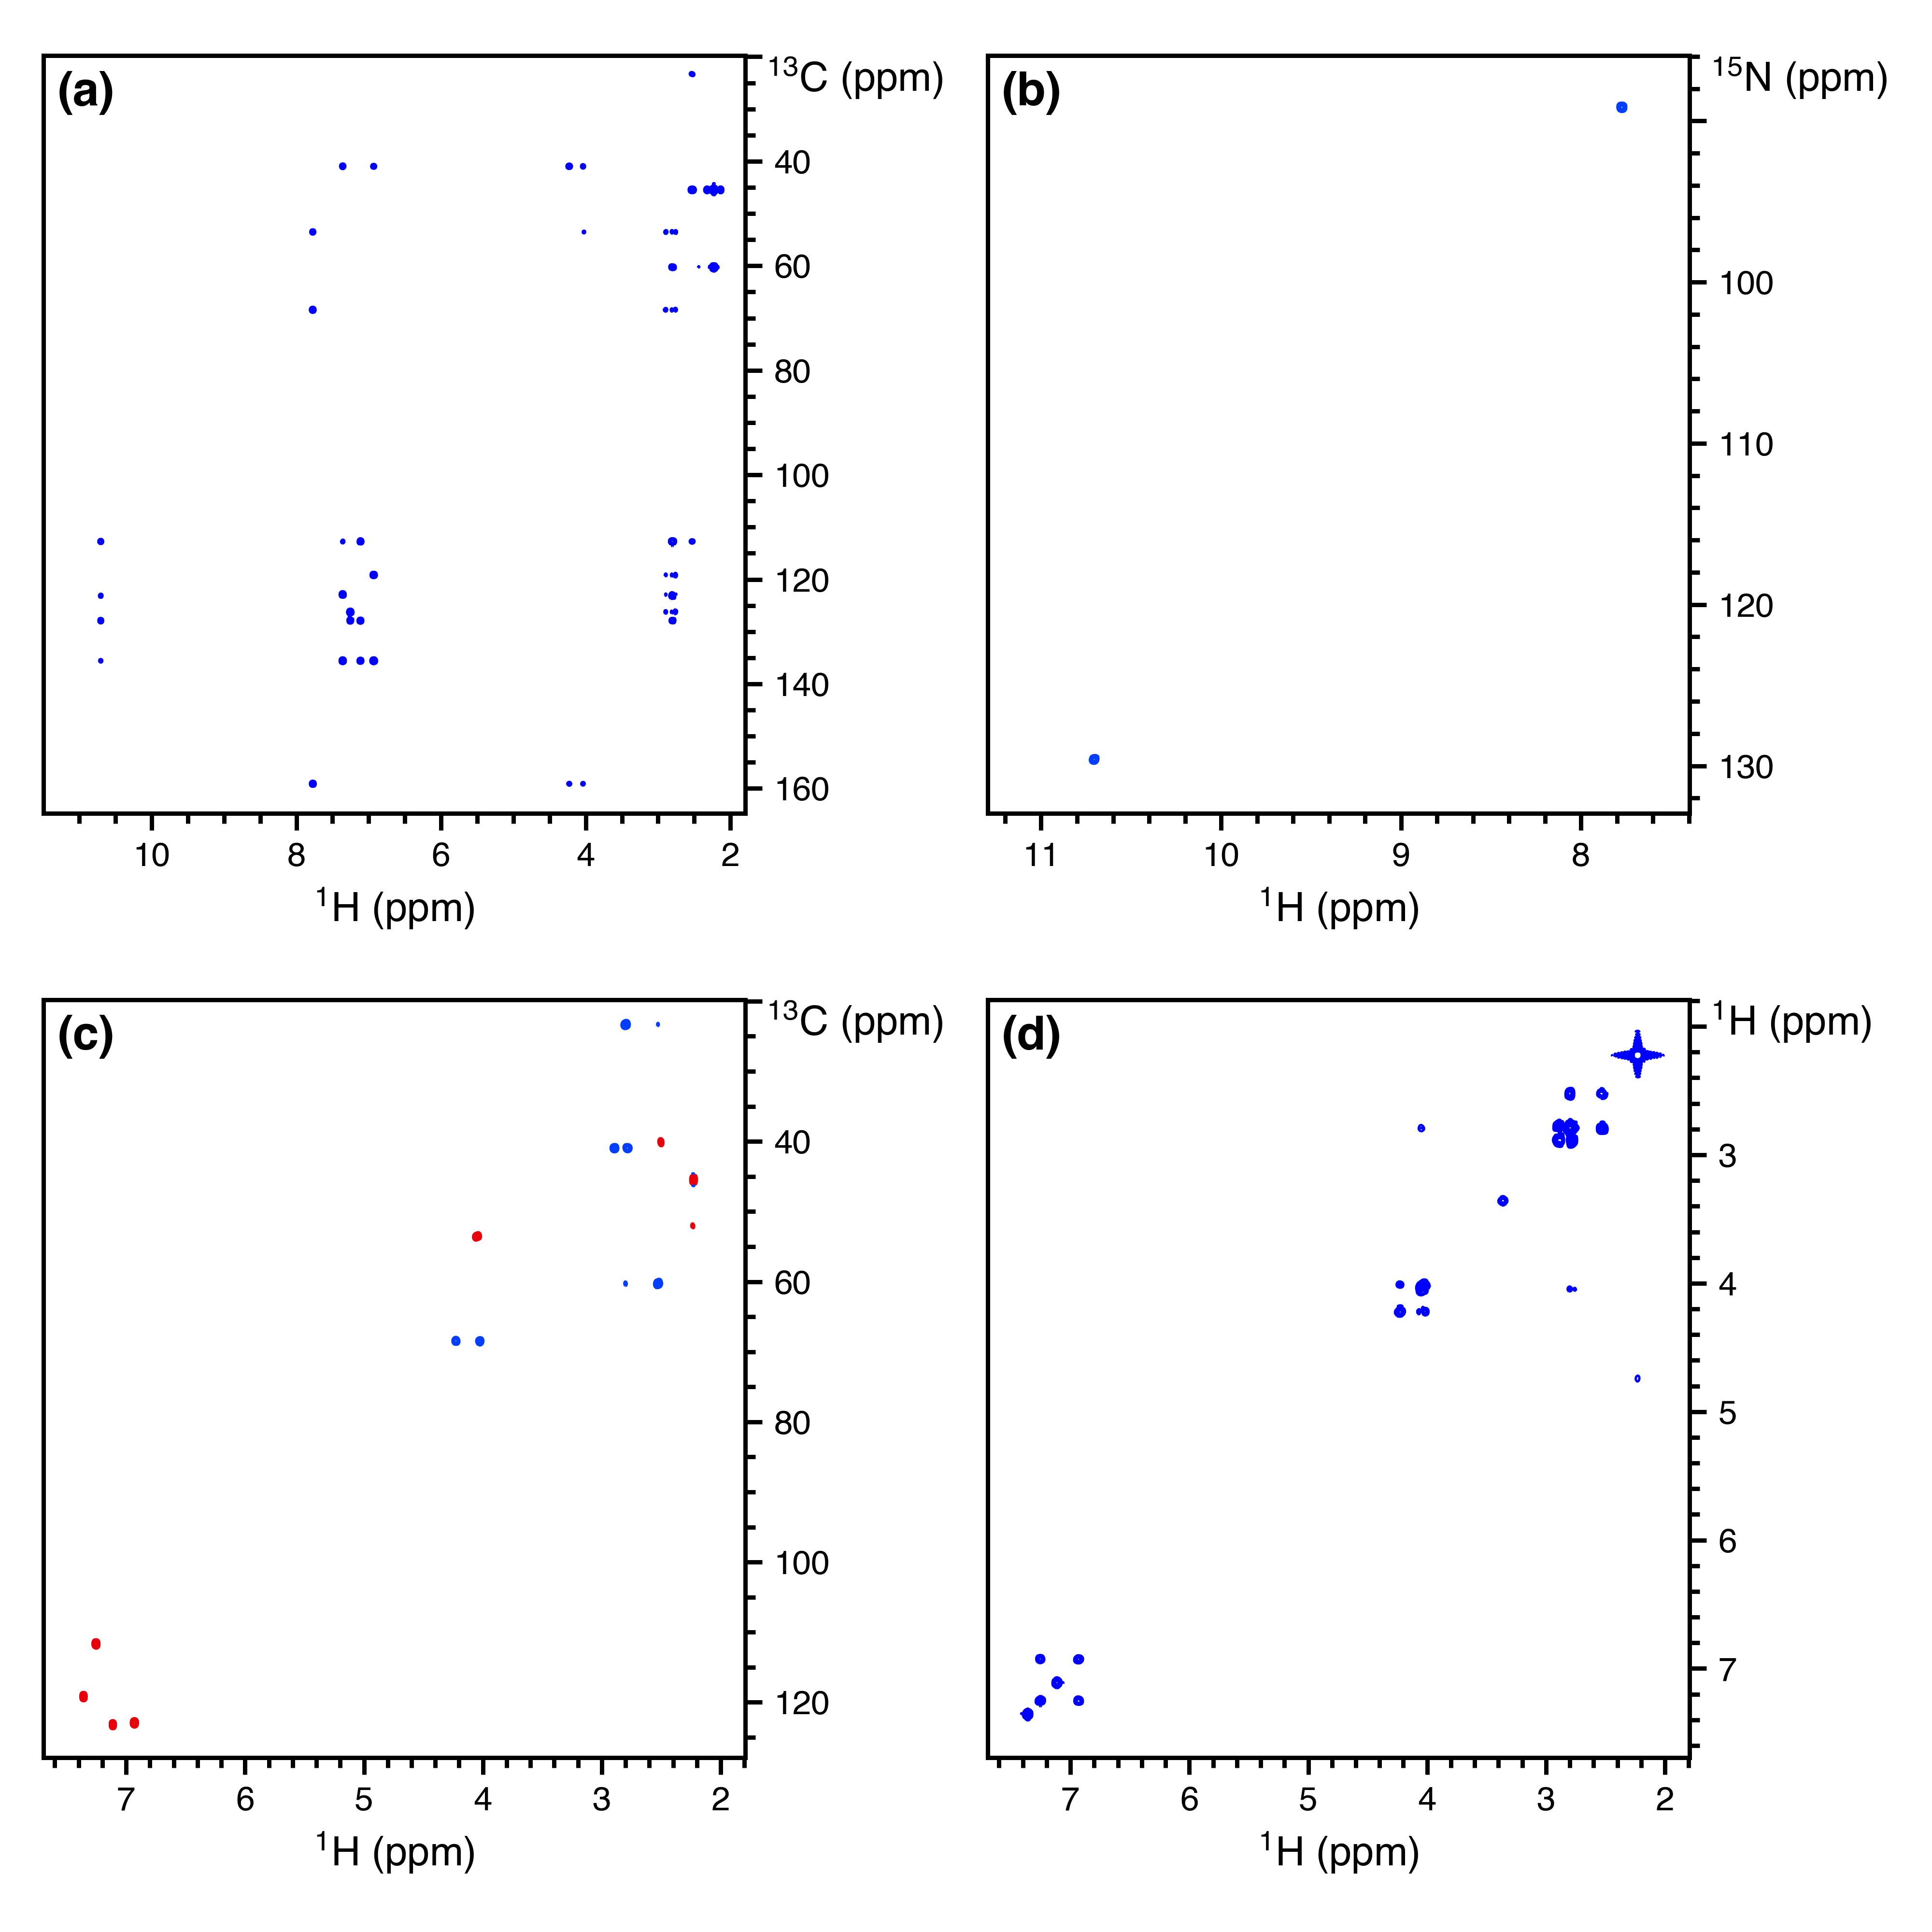
\includegraphics[width=0.8\textwidth]{./figures/bspnspcqf.png}
    \caption{
        2D spectra acquired using the NOAH-4 BSpnSpCqf supersequence.
        256 $t_1$ increments were used with 2 scans per increment, leading to a total experiment time of 17 minutes and 32 seconds.
        This represents a $3.22\times$ time saving relative to conventional acquisition of each of the four spectra with the same parameters, which would take a total of 56 minutes and 28 seconds.
        \textbf{(a)} HMBC.
        \textbf{(b)} \nitrogen{} seHSQC with $k = 4$ and linear projected to 512 complex points.
        \textbf{(c)} Multiplicity edited \carbon{} seHSQC.
        \textbf{(d)} Magnitude-mode COSY.
        \zolmi{}
    }
    \label{fig:bspnspcqf}
\end{figure}

\section{Pulse programmes}

\hl{
    I have not fleshed out this part and the next.
    Firstly, it makes the SI really really long (StSpCc is 10 pages long!!), and for not much purpose anyway:
    I am of the opinion that users are better served by downloading a file rather than copying pages of text from a PDF -- which can go quite wrong sometimes as odd characters and page numbers get copied too!
    Secondly, it is quite easy to do this up, as \LaTeX{} provides mechanisms by which the entire contents of a file can be included.
    So it can be done at a later stage.

    Alternatively, we can point people to Bruker library, or nmrweb.chem, or (depending on which journal we go to) they might allow zip files as a supplementary file.
}

\small
\singlespacing

\subsection{NOAH-2 SpCc: seHSQC + CLIP-COSY}
\verbatiminput{pulprogs/noah2-SpCc}

\subsection{NOAH-3 StSpCc: HSQC-TOCSY + seHSQC + CLIP-COSY}
\verbatiminput{pulprogs/noah3-StSpCc}

\normalsize

\section{Processing scripts}

...
